\documentclass[xcolor={dvipsnames},aspectratio=169,10pt]{beamer}
\usetheme{mx}
\usepackage{graphicx}
\graphicspath{{figures/}}
%\input{preamble.tex}

\title{
Teaching AI and Robotics to Children in a Mexican town
}
\subtitle{
Equity and Diversity in Design, Application, Methods, and Community \\
\#DEI-HRI2023 Workshop 
}

\author{
Antonio Badillo-P\'erez,
Donato Badillo-P\'erez, 
Alex Barco, \\ 
Rocio Montenegro, and
{\bf Miguel Xochicale}
}

\date{
%Workshop on Child-Robot Interaction \& Child's Fundamental Rights at 
%March 08, 2021
}

\institute{
	\faEnvelope \space  air4children@gmail.com \\
	\faGithubAlt \space @air4children \faTwitter \space @air4children  
		}

\titlegraphic{
  \begin{tikzpicture}[overlay, remember picture]
    \node[%
      above right=0.35cm and -0.2cm of current page footer area.south west,
      anchor=south west,
      inner sep=0pt] {%
      \usebeamerfont{footline}
      \begin{tabular}{lm{.8\textwidth}}
        \href{http://creativecommons.org/licenses/by/4.0/}{\ccby} &
        This slices is licensed under a
	\href{http://creativecommons.org/licenses/by/4.0/}
		{Creative Commons ``Attribution 4.0 International''} license. 
	\par Get source of this slides and see further references 
		from \url{https://github.com/air4children/dei-hri2023}.
      \end{tabular}
    };
    \node[%
      above left=0.35cm and 0cm of current page footer area.south east,
      anchor=south east,
      inner sep=0pt]{\qrcode[height=1.5cm]{https://github.com/air4children/dei-hri2023}};
  \end{tikzpicture}
}

\begin{document}

\maketitle

\begin{frame}{Table of Contents}
    \tableofcontents
\end{frame}

%%%%%%%%%%%%%%%%%%%%%%%%%%%%%%%%%%%%%%%%%%%%
\section{Background}


\begin{frame}
      \frametitle{Table of Contents}
      \tableofcontents[currentsection]
\end{frame}



%%%%%%%%%%%%%%%%%%%%%%%%%%%%%%%%%%%%%%%%%%%%%
\subsection{Education programs, publications and private investment in AI and Robotics}

%%%%%%%%%%%%%%%%%%%%%%%%%%%%%%%%%%%%%%%%%%%%%%%%%%%%%%%%
{
%\paper{Savage N. 2021 in Nature, DOI: doi.org/10.1038/d41586-020-03409-8}
\paper{Zhang D. et al 2021 in AI 2021 Index Report, Fig 4.3.3 https://aiindex.stanford.edu/report/}

\begin{frame}{Specialised AI programs by Geographic Area and level}

\begin{figure}
 \centering
 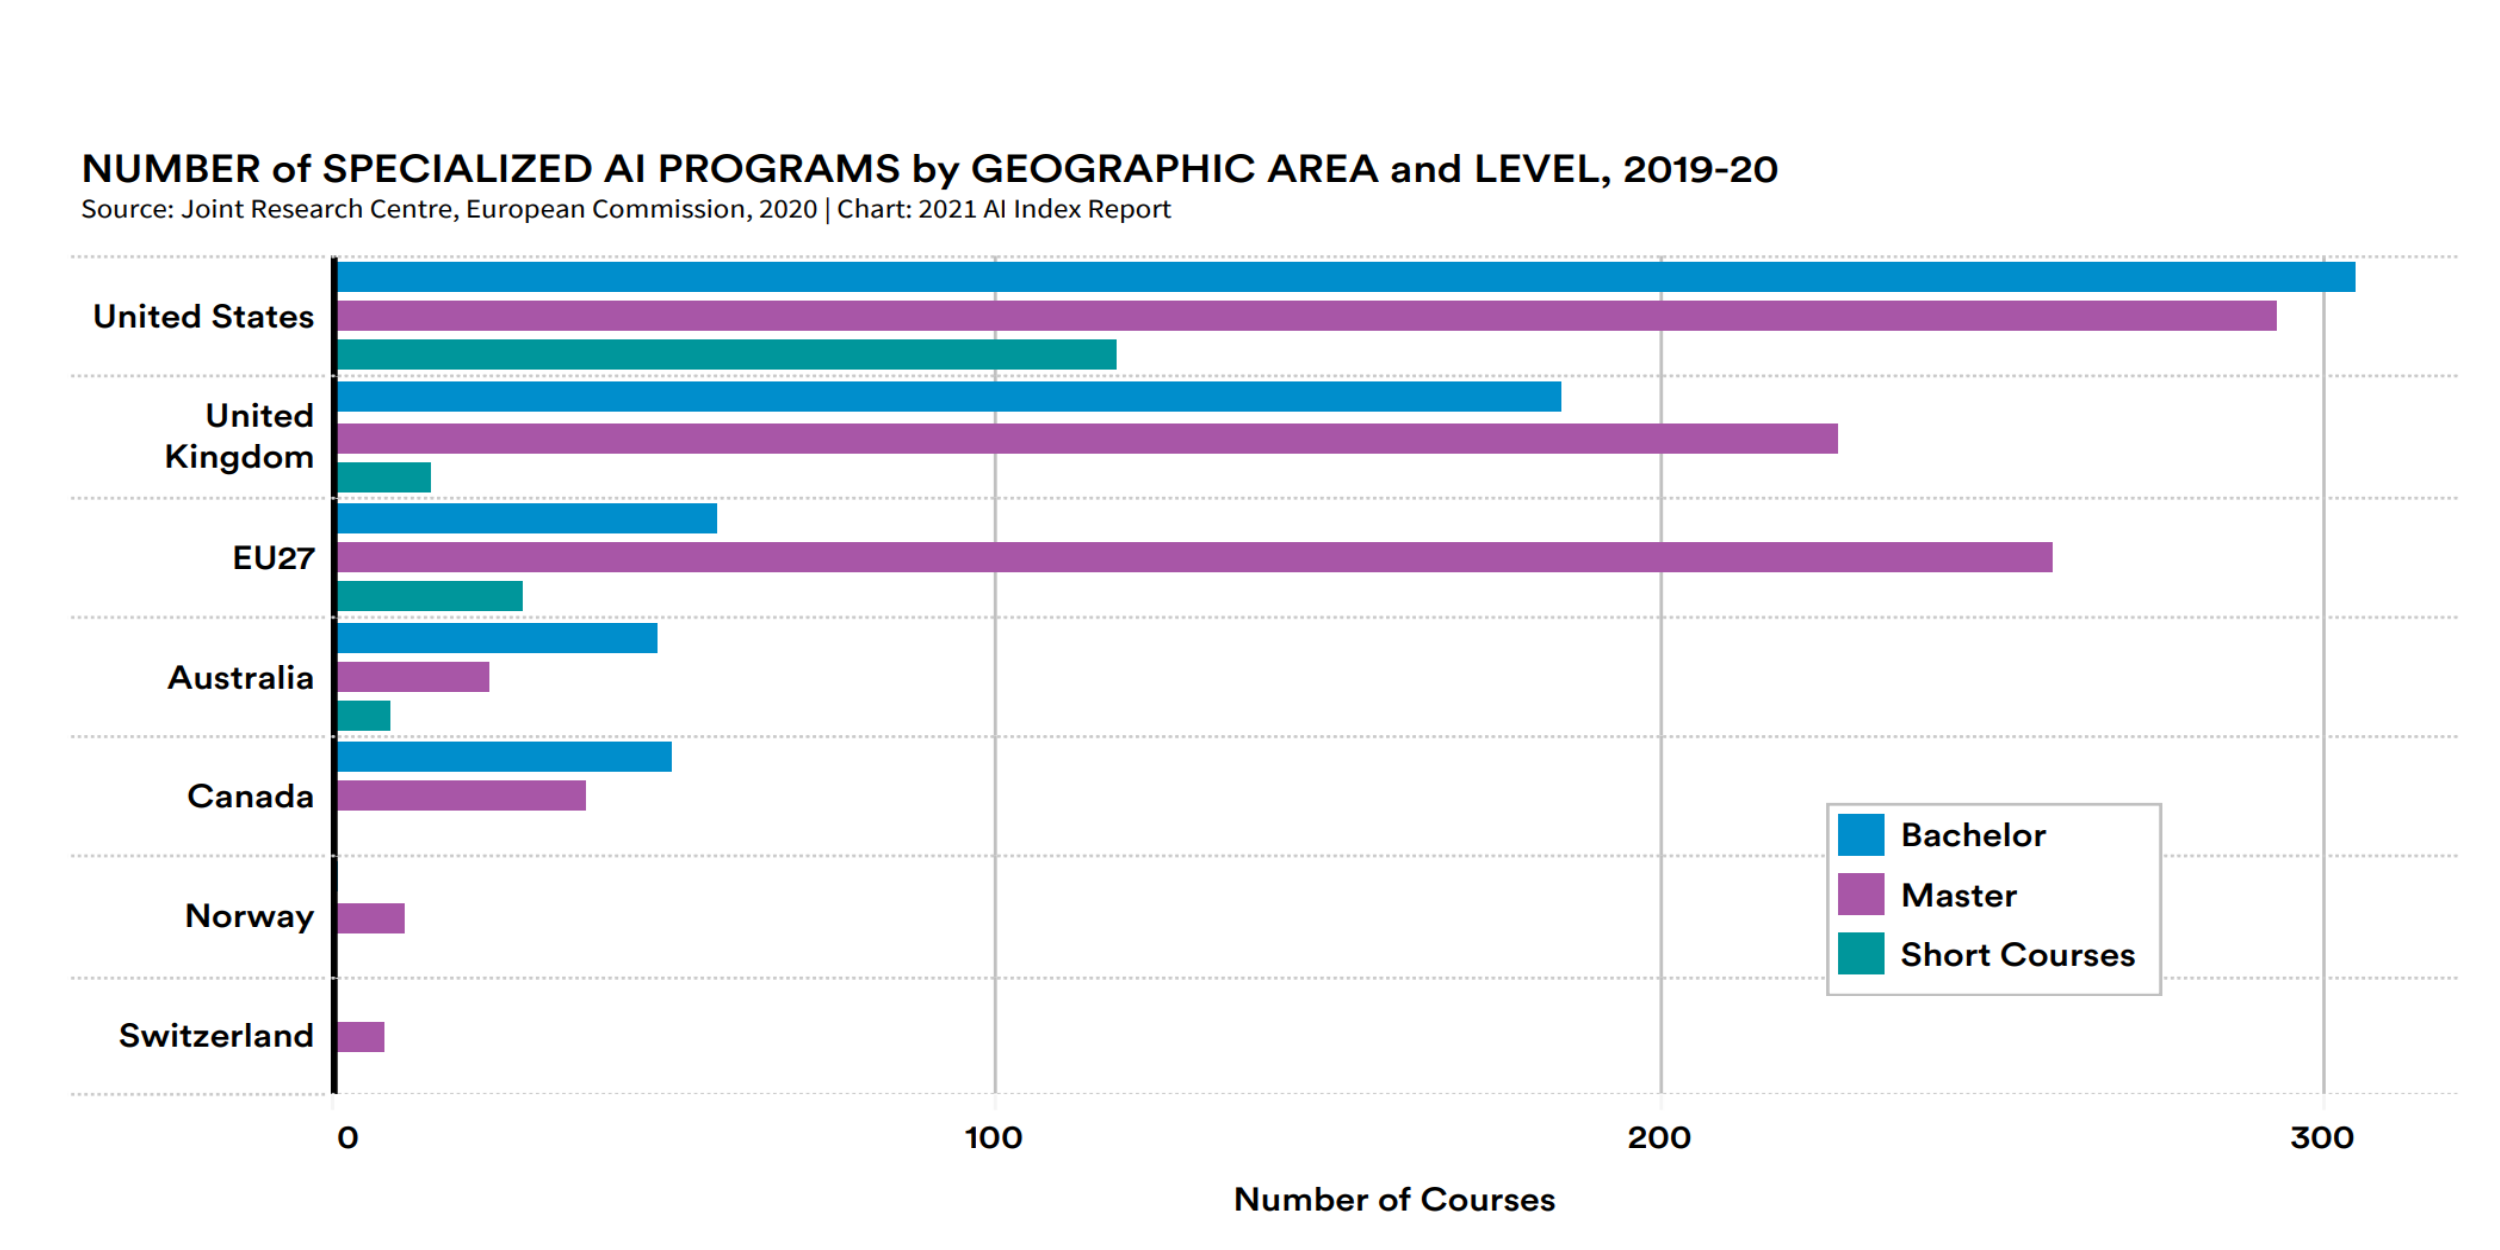
\includegraphics[width=1.0\textwidth]{./figures/progress-of-air-a/outputs/drawing-v00.png}
 %\caption{}
\end{figure}

\end{frame}
}


%%%%%%%%%%%%%%%%%%%%%%%%%%%%%%%%%%%%%%%%%%%%%%%%%%%%%%%%
{
%\paper{Savage N. 2021 in Nature, DOI: doi.org/10.1038/d41586-020-03409-8}
\paper{Zhang D. et al 2021 in AI 2021 Index Report, Fig 1.1.19 https://aiindex.stanford.edu/report/}

\begin{frame}{AI-related publications in arxiv by field of study}

\begin{figure}
 \centering
 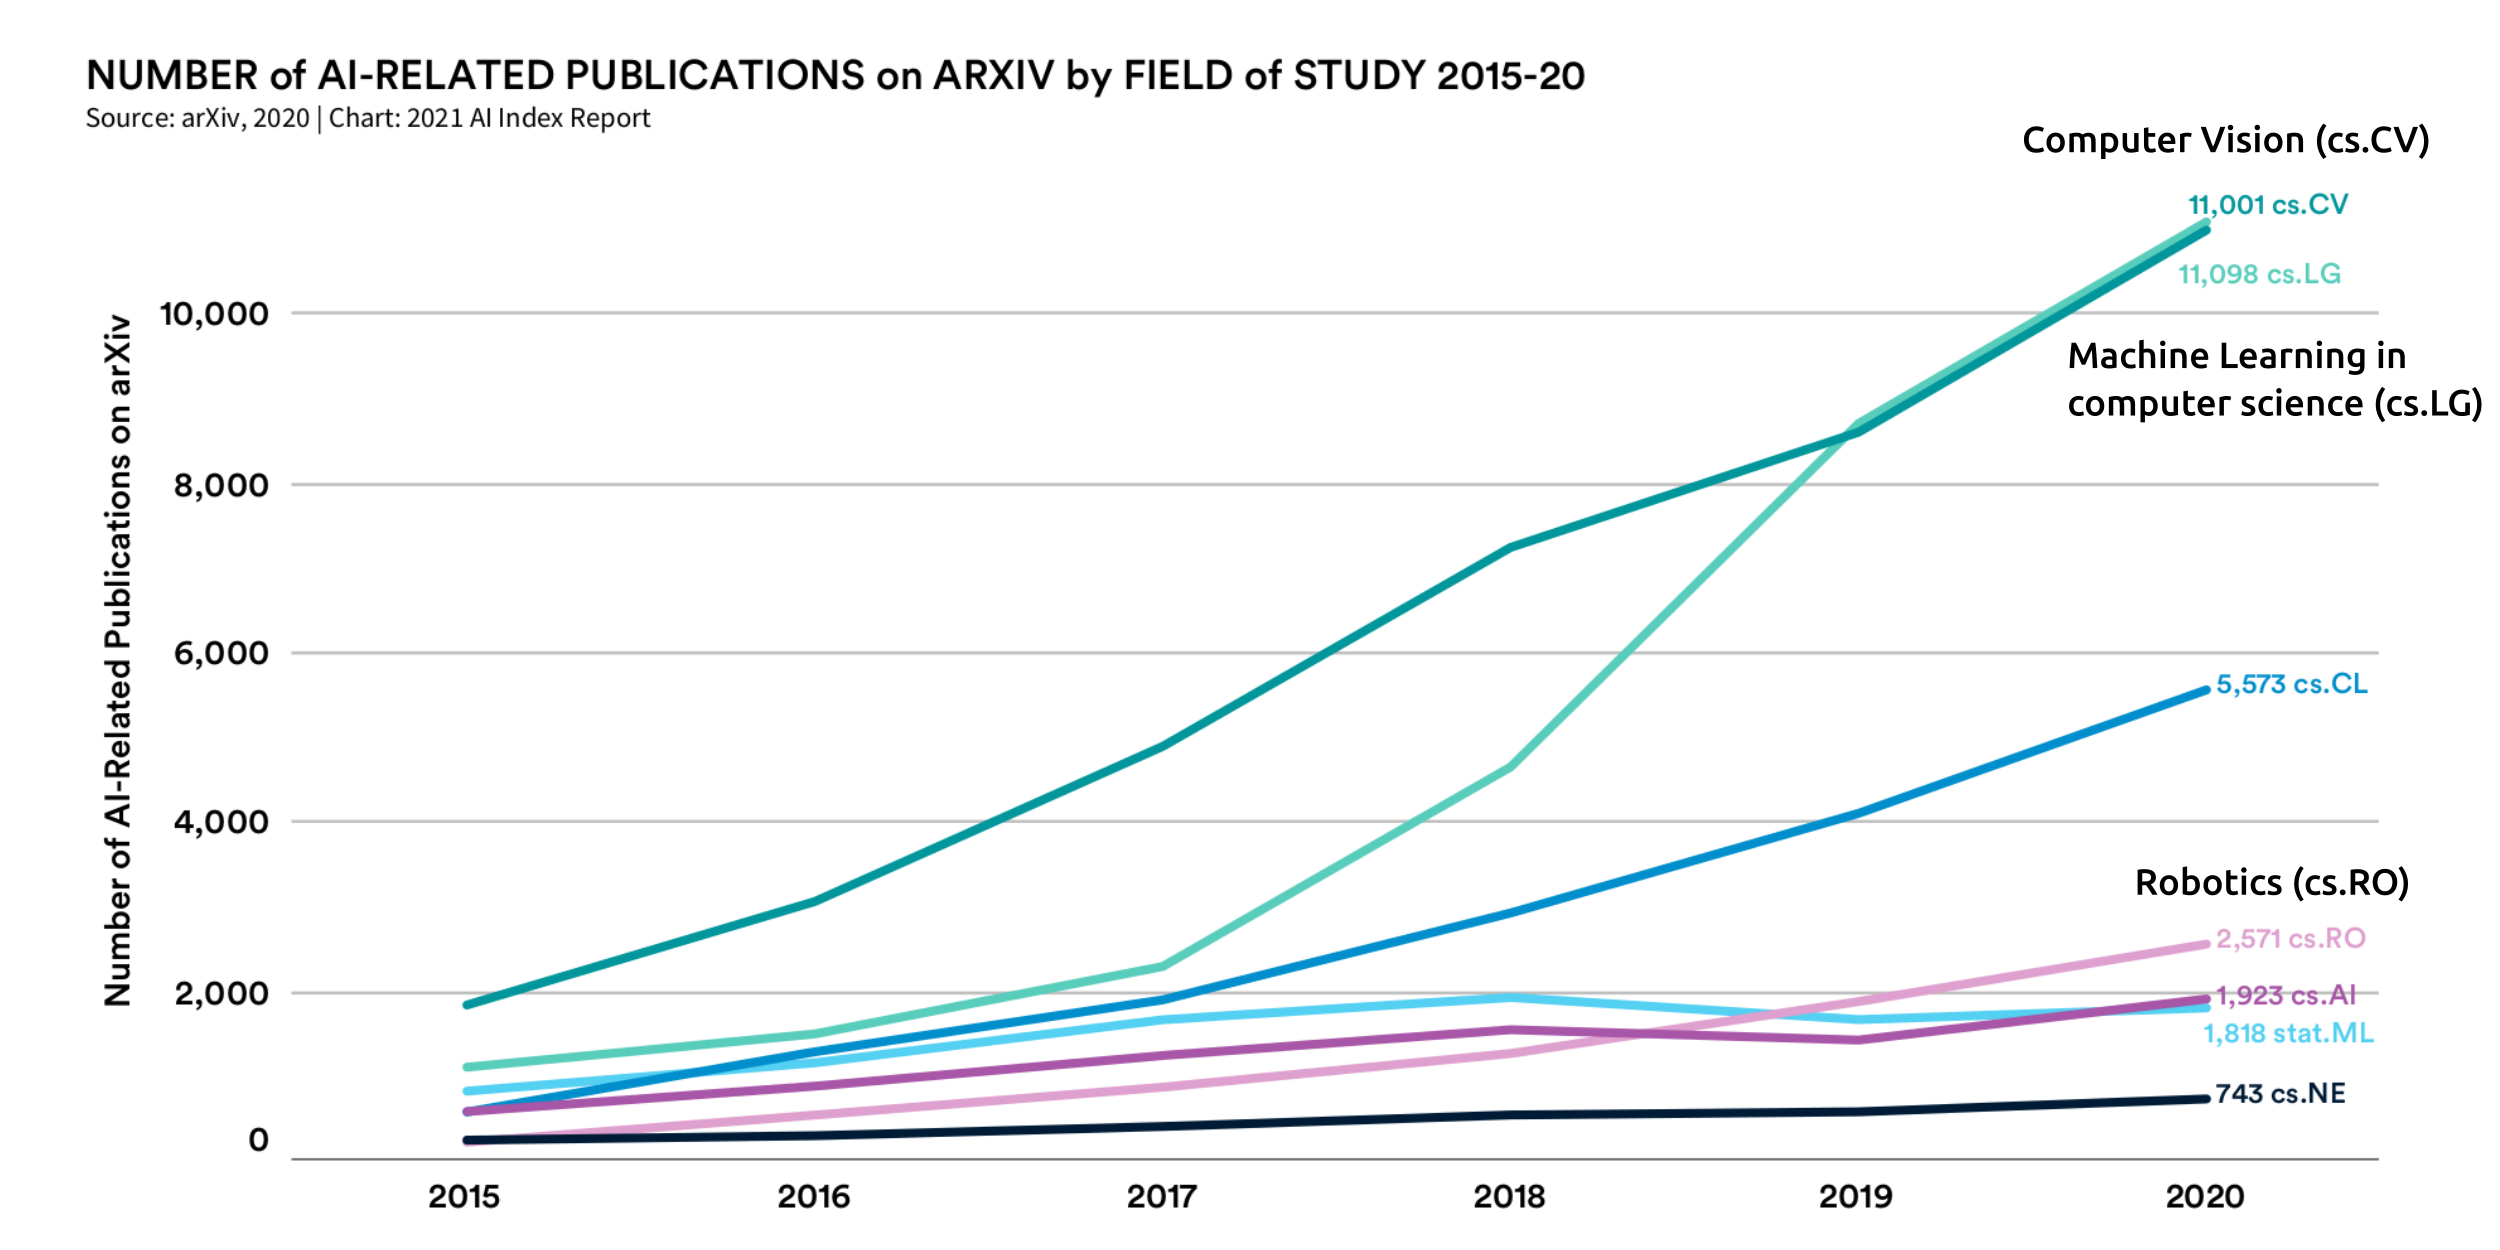
\includegraphics[width=1.0\textwidth]{./figures/progress-of-air-b/outputs/drawing-v00.png}
 %\caption{}
\end{figure}

\end{frame}
}



%%%%%%%%%%%%%%%%%%%%%%%%%%%%%%%%%%%%%%%%%%%%%%%%%%%%%%%%
{
%\paper{Savage N. 2021 in Nature, DOI: doi.org/10.1038/d41586-020-03409-8}
\paper{Zhang D. et al 2021 in AI 2021 Index Report, Fig 1.1.19 https://aiindex.stanford.edu/report/}

\begin{frame}{Private investment in AI by Geographic area}

\begin{figure}
 \centering
 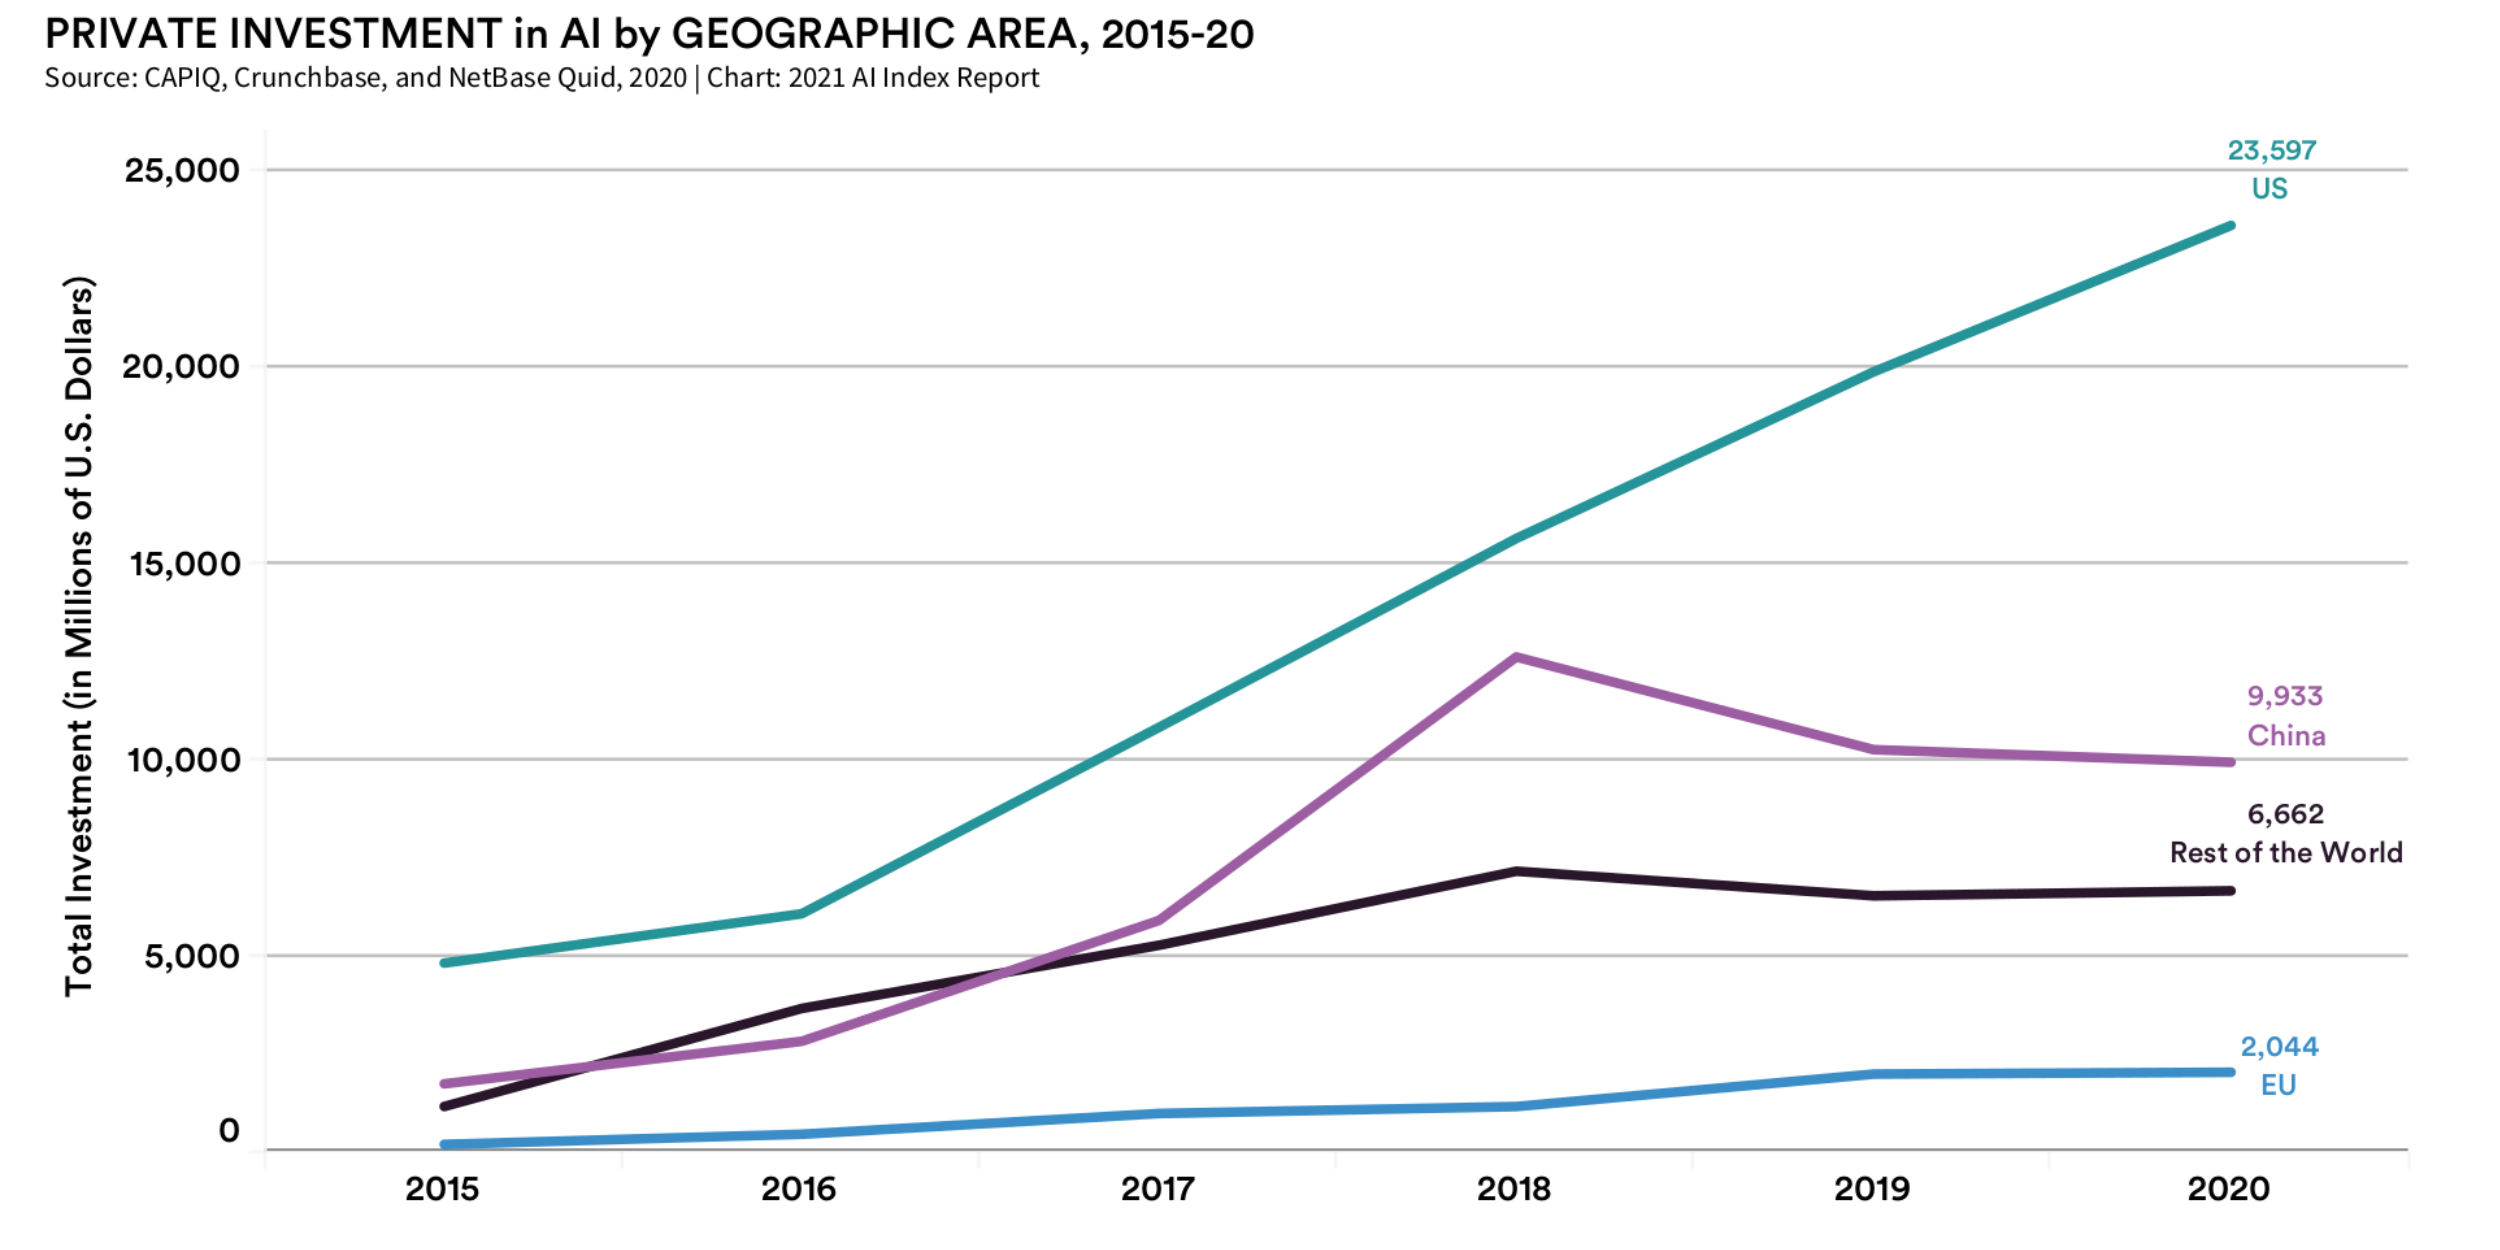
\includegraphics[width=1.0\textwidth]{./figures/progress-of-air-c/outputs/drawing-v00.png}
 %\caption{}
\end{figure}

\end{frame}
}



%%%%%%%%%%%%%%%%%%%%%%%%%%%%%%%%%%%%%%%%%%%%%
\subsection{Open source software and hardware in AI and Robotics}

%%%%%%%%%%%%%%%%%%%%%%%%%%%%%%%%%%%%%%%%%%%%%%%%%%%%%%%%
{
%\paper{Savage N. 2021 in Nature}
\begin{frame}{Open source software and hardware in AI and Robotics}

      \begin{figure}
        \centering
        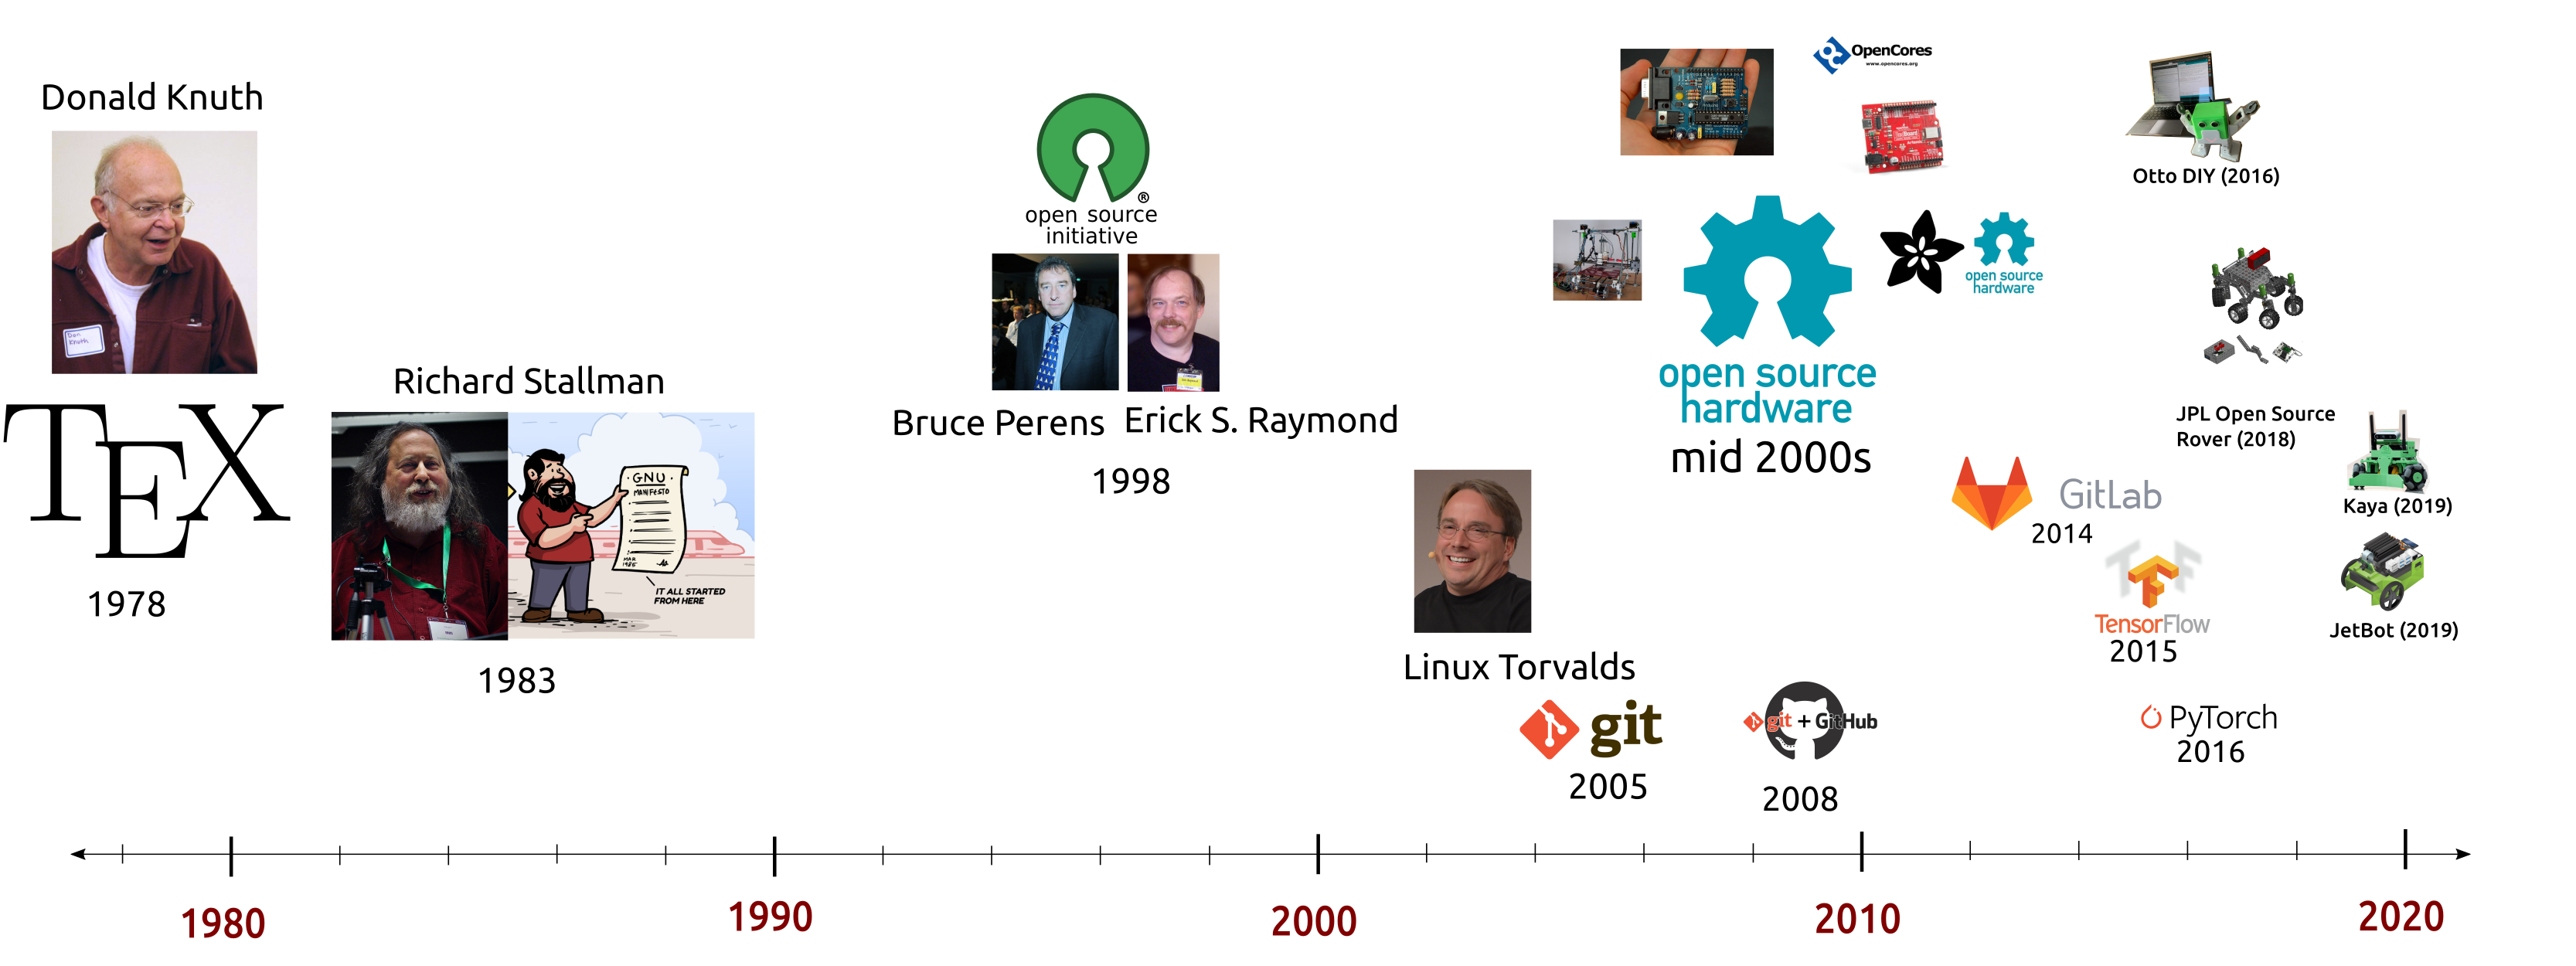
\includegraphics[width=1.0\textwidth]{./figures/timeline-osh/outputs/drawing-v00.png}
        %\caption{}
      \end{figure}
\end{frame}
}


%%%%%%%%%%%%%%%%%%%%%%%%%%%%%%%%%%%%%%%%%%%%
\section{air4children}


\begin{frame}
      \frametitle{Table of Contents}
      \tableofcontents[currentsection]
\end{frame}


%%%%%%%%%%%%%%%%%%%%%%%%%%%%%%%%%%%%%%%%%%%%%%%%%%%%%%%%
{
%\paper{Lastname N. YEAR in journal of...}
\begin{frame}{What is air4children?}

  \begin{columns}
  \begin{column}{.7\linewidth}

  air4children, Artificial Intelligence and Robotics for Children, aiming  
  \begin{itemize}
    \item to create a more inclusive, affordable and fair participation of children in AI and Robotics,
    \item to create child-centred AI and Robotics curriculums based on Montessori Education, and
    \item to build Open source robots to be affordable and fun. 
  \end{itemize}

    \end{column}


  \begin{column}{.4\linewidth}

      \begin{figure}
        \centering
        
\includegraphics[width=0.95\textwidth]{./figures/logo/outputs/drawing-v00.png}
      \end{figure}

    \end{column}
  \end{columns}

\end{frame}
}




%%%%%%%%%%%%%%%%%%%%%%%%%%%%%%%%%%%%%%%%%%%%%
\subsection{Prototyping and piloting Open Source Robots}

%%%%%%%%%%%%%%%%%%%%%%%%%%%%%%%%%%%%%%%%%%%%%%%%%%%%%%%%
{
\paper{Xochicale M. 2014, \it{Proposal of Libre Robotics} }
\begin{frame}{Prototyping Open Source Robots (2013 -- 2017)}
      \begin{figure}
        \centering
        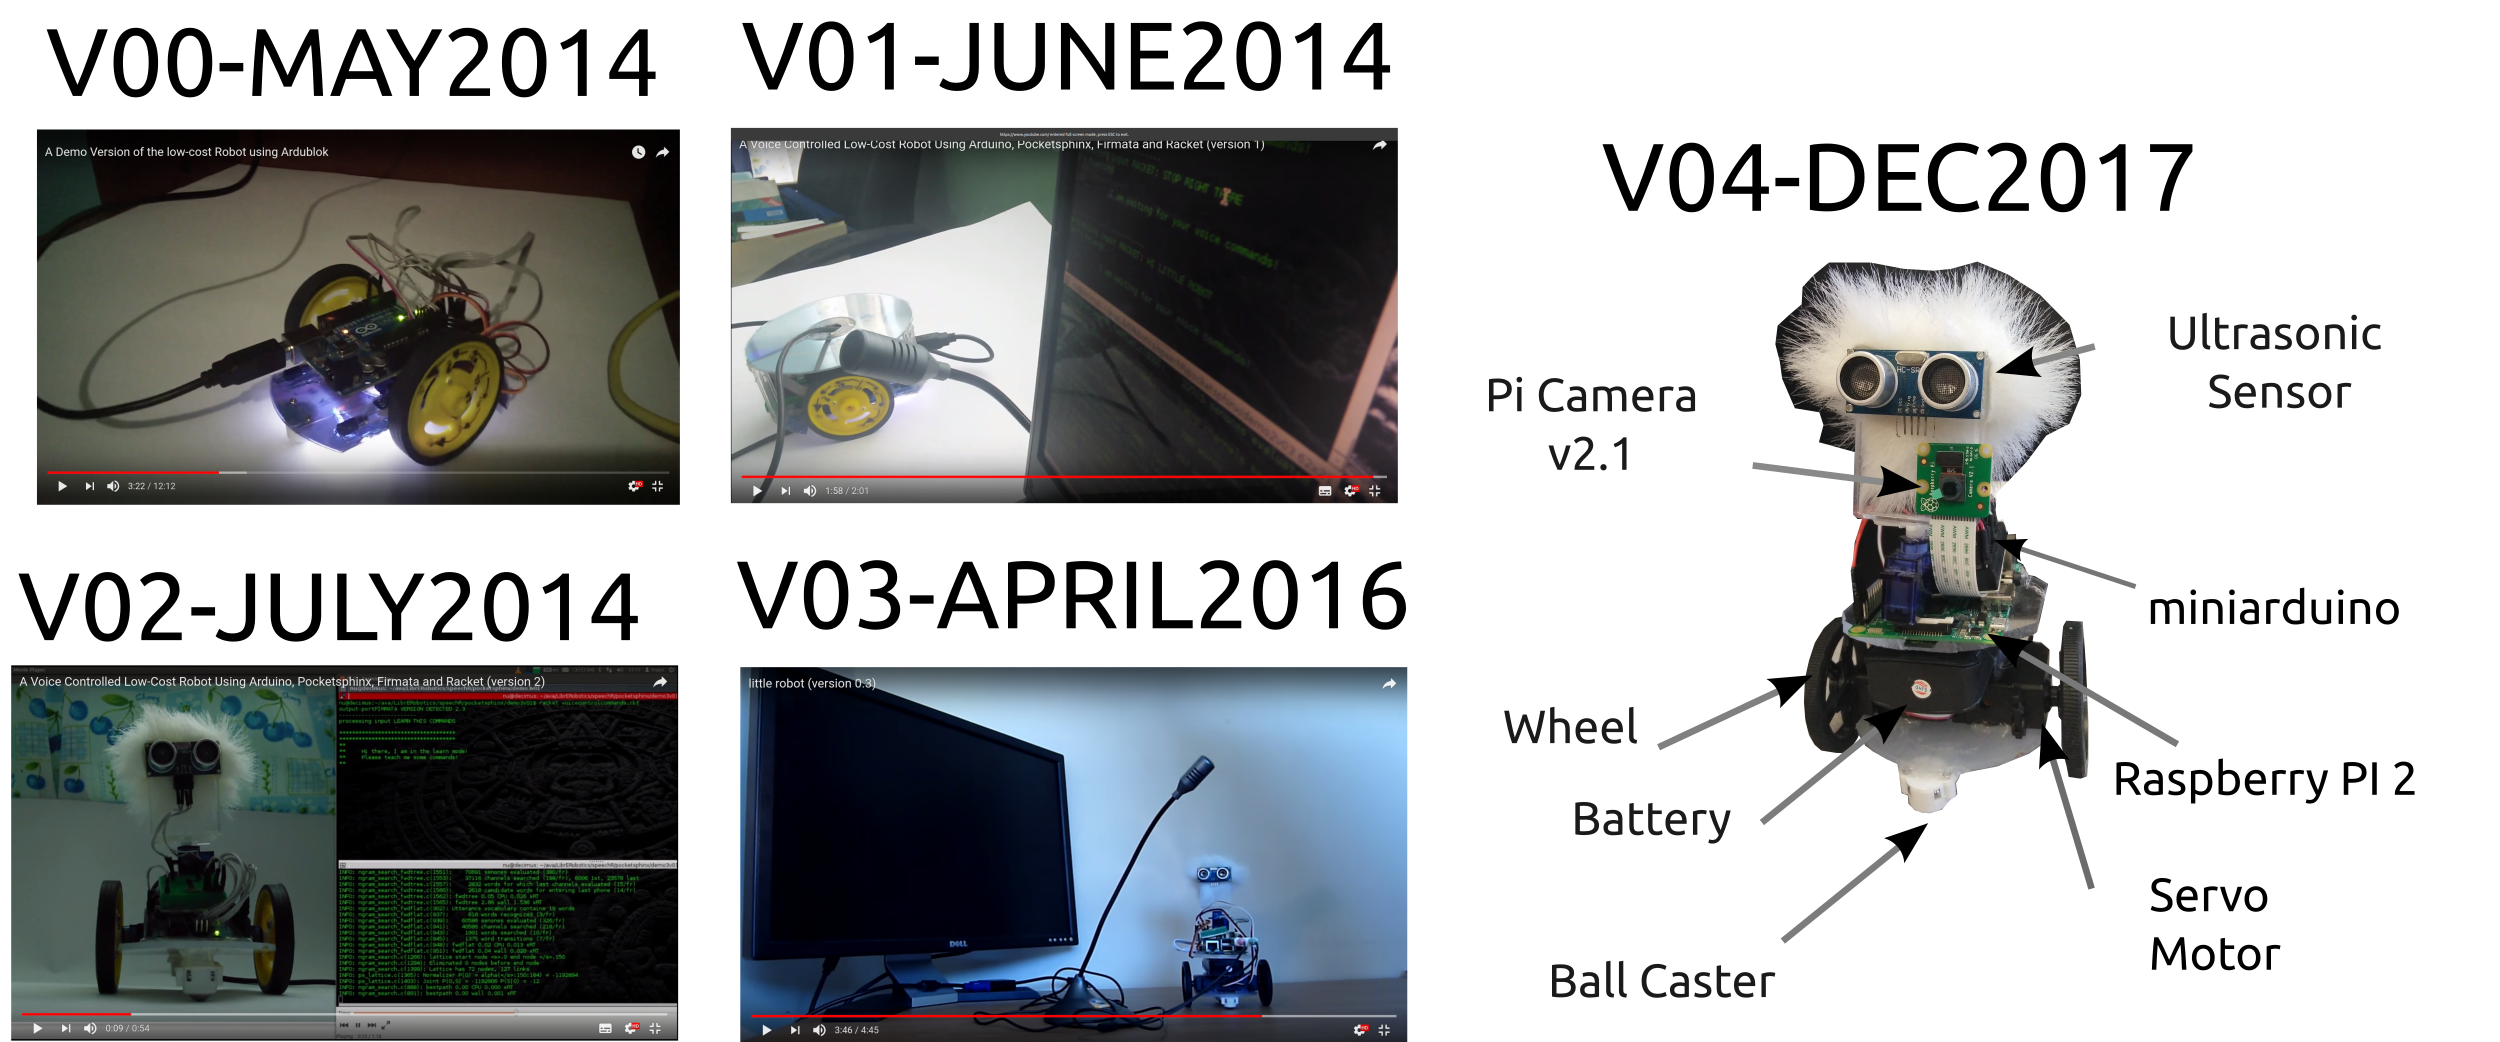
\includegraphics[width=1.0\textwidth]{./figures/air4children-a/outputs/drawing-v00.png}
        %\caption{}
      \end{figure}
\end{frame}
}

%%%%%%%%%%%%%%%%%%%%%%%%%%%%%%%%%%%%%%%%%%%%%%%%%%%%%%%%
{
\paper{Xochicale M. 2015 in Mecate; Parra C. et al. 2016, \it{Otto DIY}}
\begin{frame}{Piloting robot prototypes (2015 -- 2019)}
      \begin{figure}
        \centering
        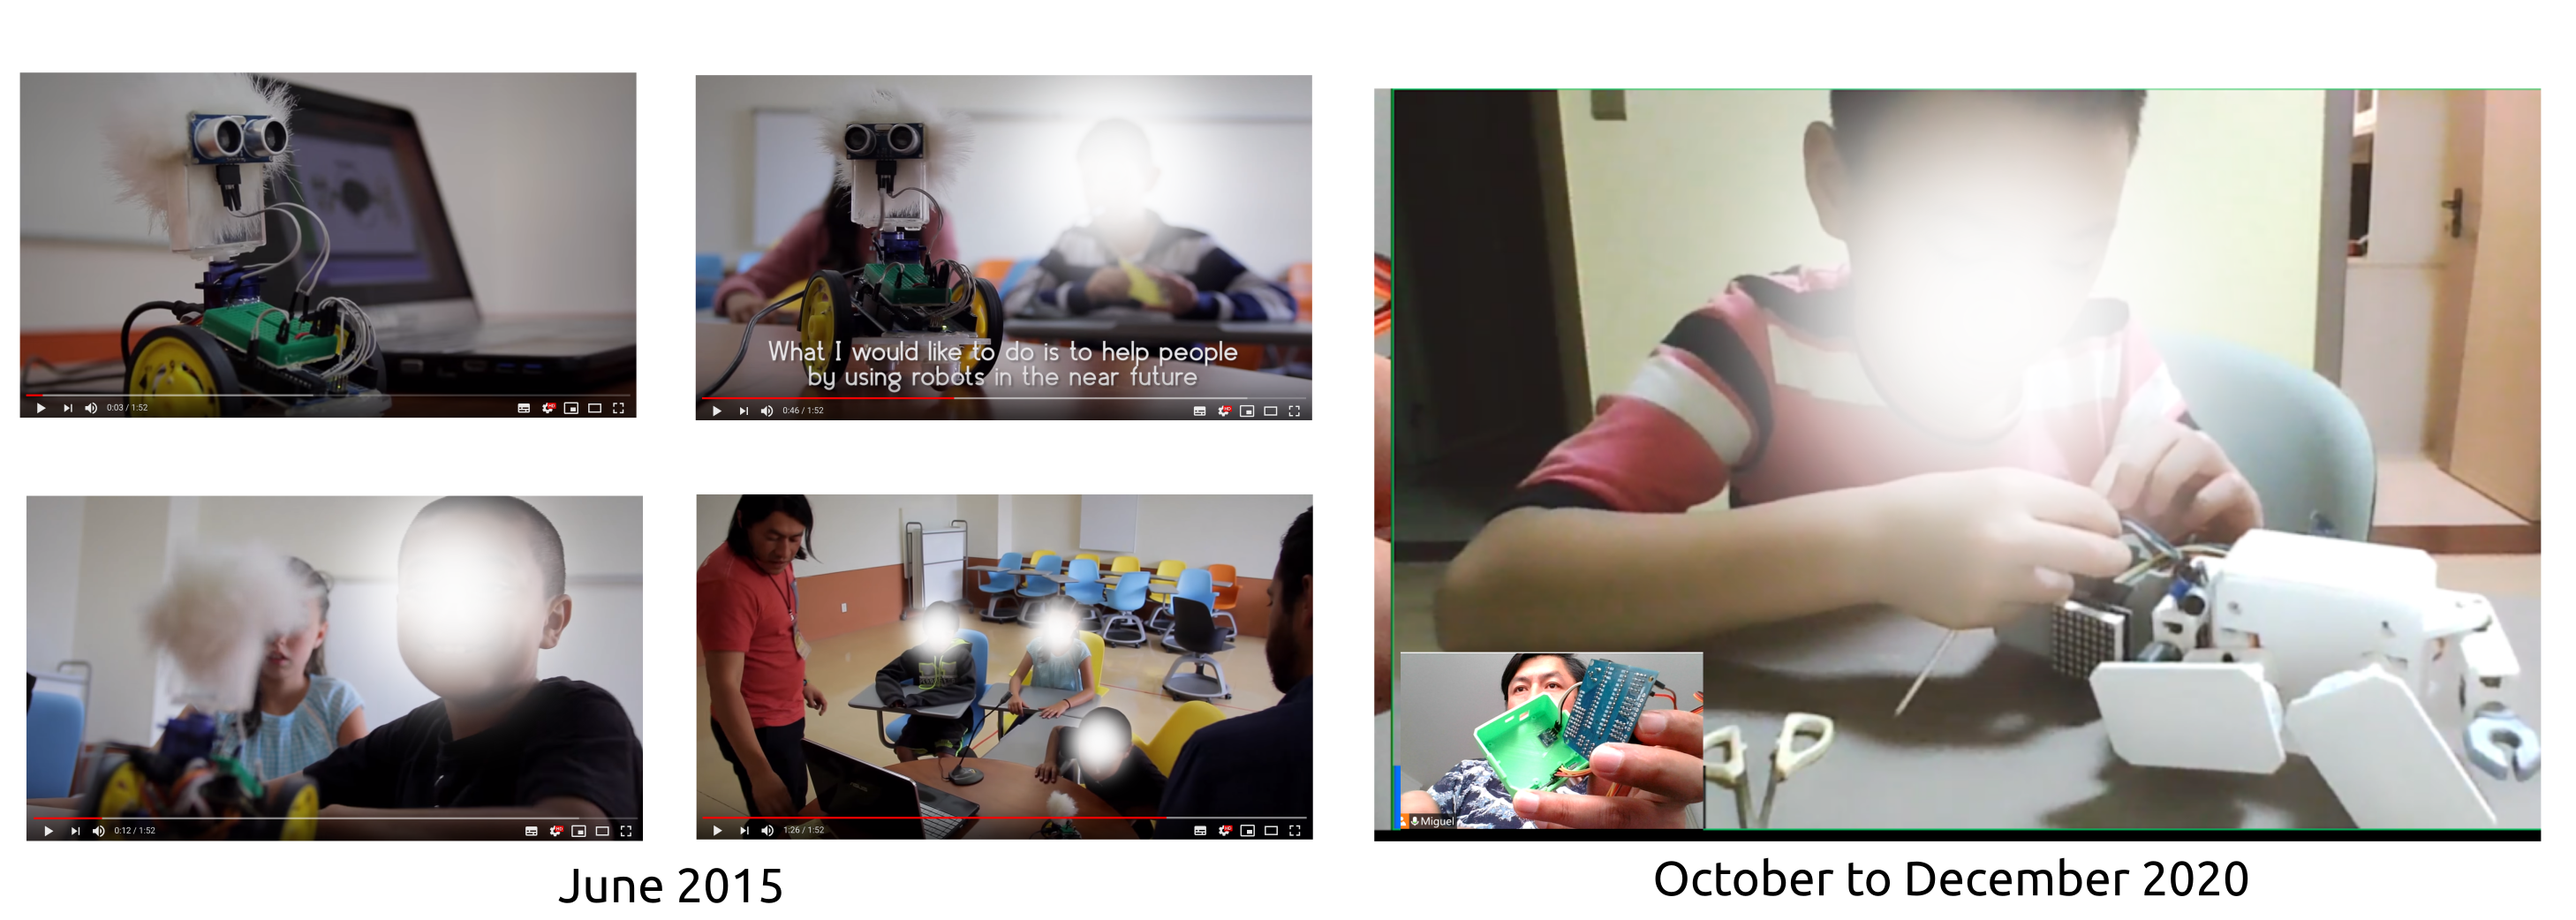
\includegraphics[width=1.0\textwidth]{./figures/air4children-b/outputs/drawing-v00.png}
        %\caption{}
      \end{figure}
\end{frame}
}

%%%%%%%%%%%%%%%%%%%%%%%%%%%%%%%%%%%%%%%%%%%%%
\subsection{Montessori Education}

%%%%%%%%%%%%%%%%%%%%%%%%%%%%%%%%%%%%%%%%%%%%%%%%%%%%%%%%
{
\paper{Elkin M., Sullivan A, Bers 2014 in Journal of Information and Technology}
\begin{frame}{Montessori Education} 
\vspace{3mm}
%\it{
"The hand is the instrument of the mind."
%} 
%\\
Dr. Maria Montessori (1970-1952).

\vspace{2mm}
    \begin{figure}
        \centering
        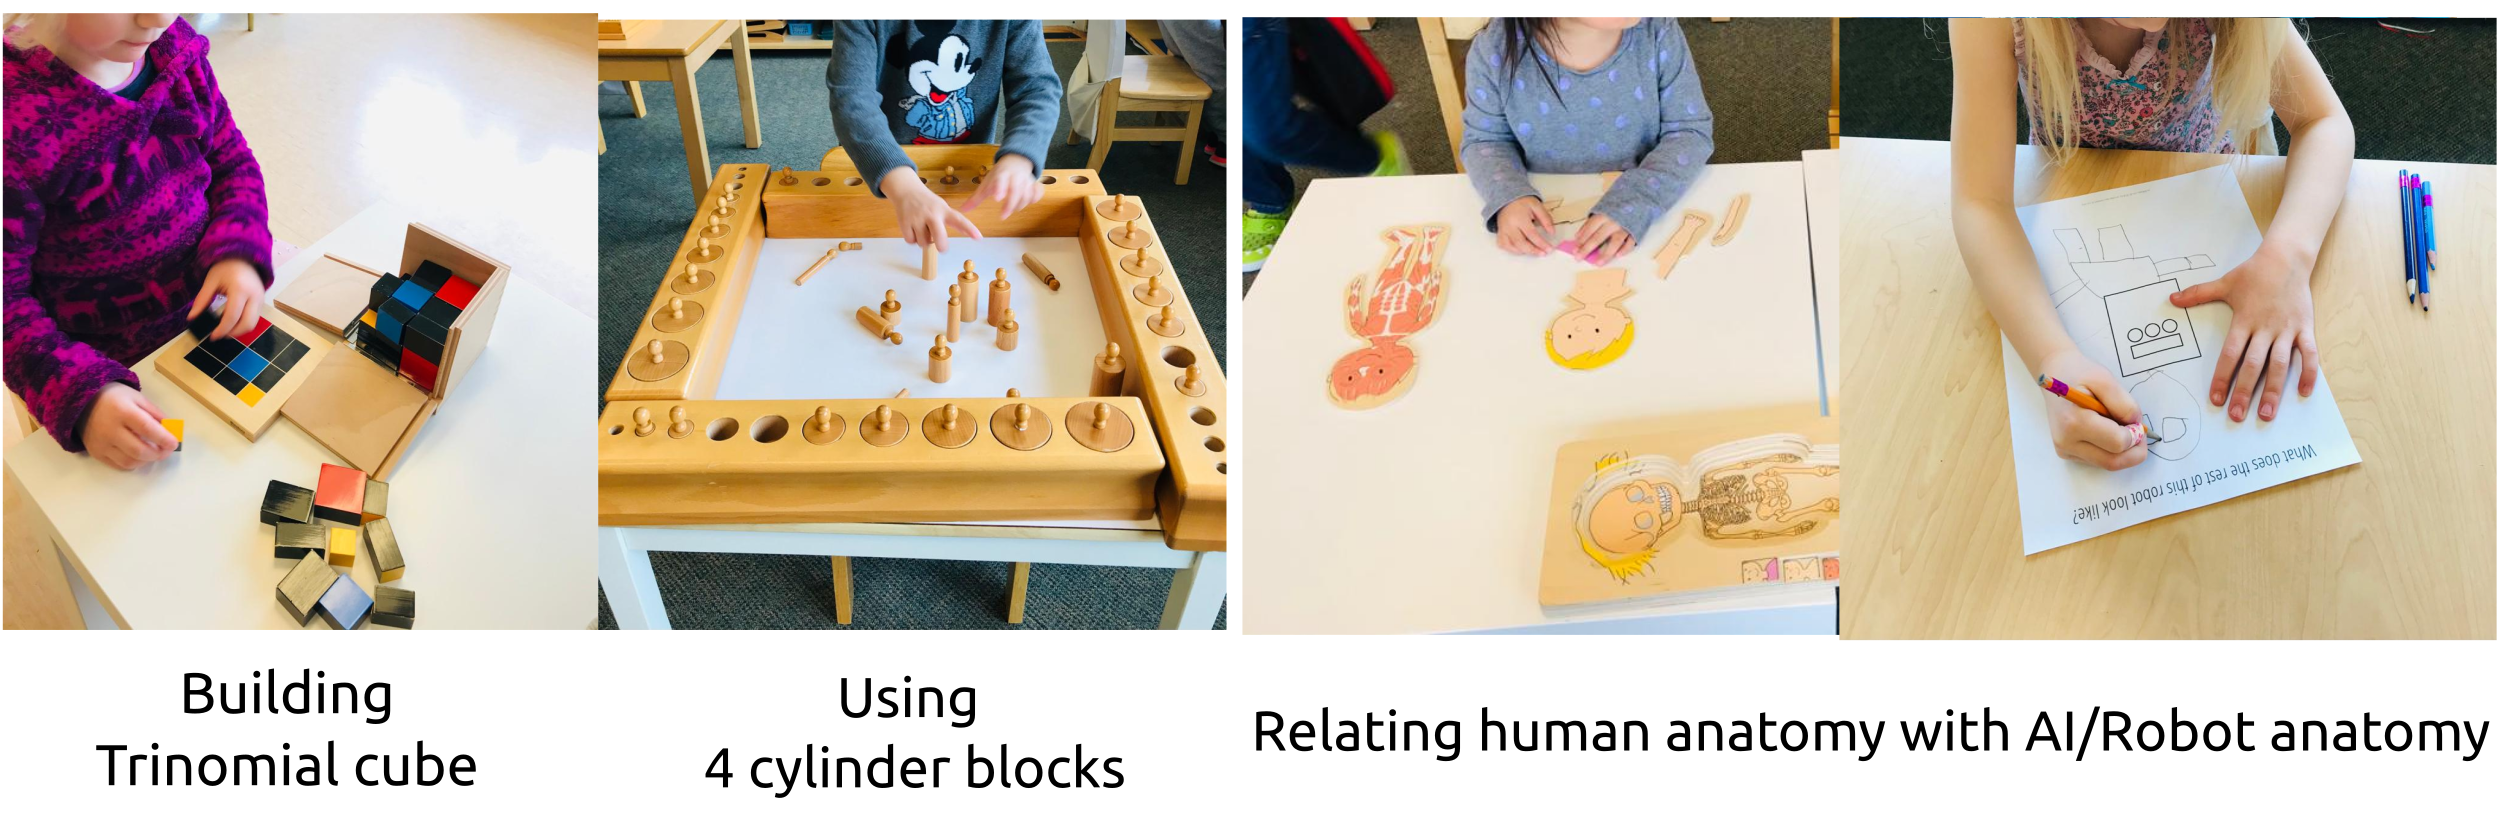
\includegraphics[width=1.0\textwidth]{./figures/montessori/outputs/drawing-v00.png}
        %\caption{}
      \end{figure}

Children are participating in creative explorations to develop fine motor skills and to engage in collaborative and teamwork activities. 

\end{frame}
}



%%%%%%%%%%%%%%%%%%%%%%%%%%%%%%%%%%%%%%%%%%%%%%%%%%%%%%%%
{
\paper{Mohammad T. et al., 2017; Harden R. M. 1999 in Journal of Medical Teacher}
\begin{frame}{Spiral Learning Method}

  \begin{figure}
        \centering
        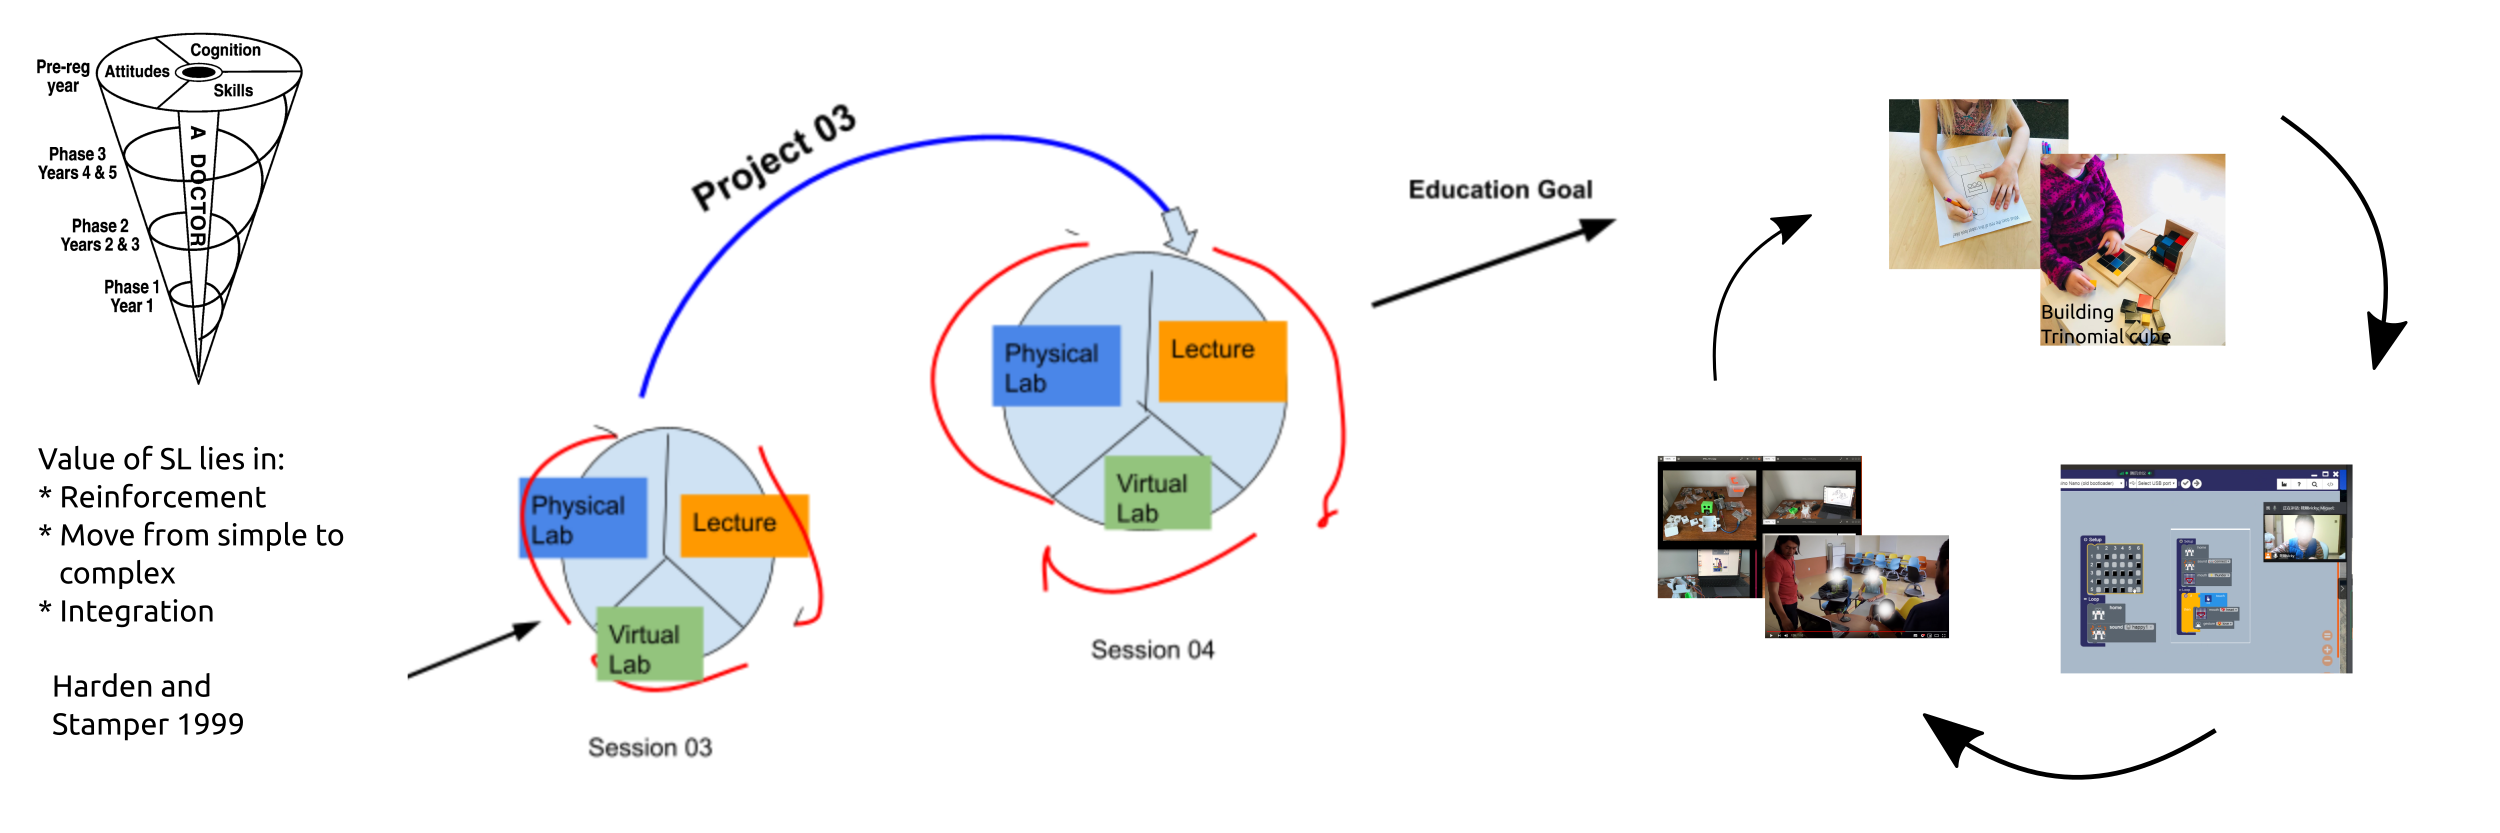
\includegraphics[width=1.0\textwidth]{./figures/teaching-materials/outputs/drawing-v02.png}
        %\caption{}
      \end{figure}
\end{frame}
}

%%%%%%%%%%%%%%%%%%%%%%%%%%%%%%%%%%%%%%%%%%%%
\section{Workshops}


\begin{frame}
      \frametitle{Table of Contents}
      \tableofcontents[currentsection]
\end{frame}




%%%%%%%%%%%%%%%%%%%%%%%%%%%%%%%%%%%%%%%%%%%%%
\subsection{Four-lesson Curriculum}

%%%%%%%%%%%%%%%%%%%%%%%%%%%%%%%%%%%%%%%%%%%%%%%%%%%%%%%%
{
\paper{Badillo-Perez A, Badillo-Perez D, Barco A, Montenegro R, Xochicale M. 2013, Teaching AI and Robotics to Children in a Mexican town, DEI-HRI2023, \url{https://arxiv.org/abs/2303.03956}}

\begin{frame}{Curriculum}
      \begin{figure}
        \centering
        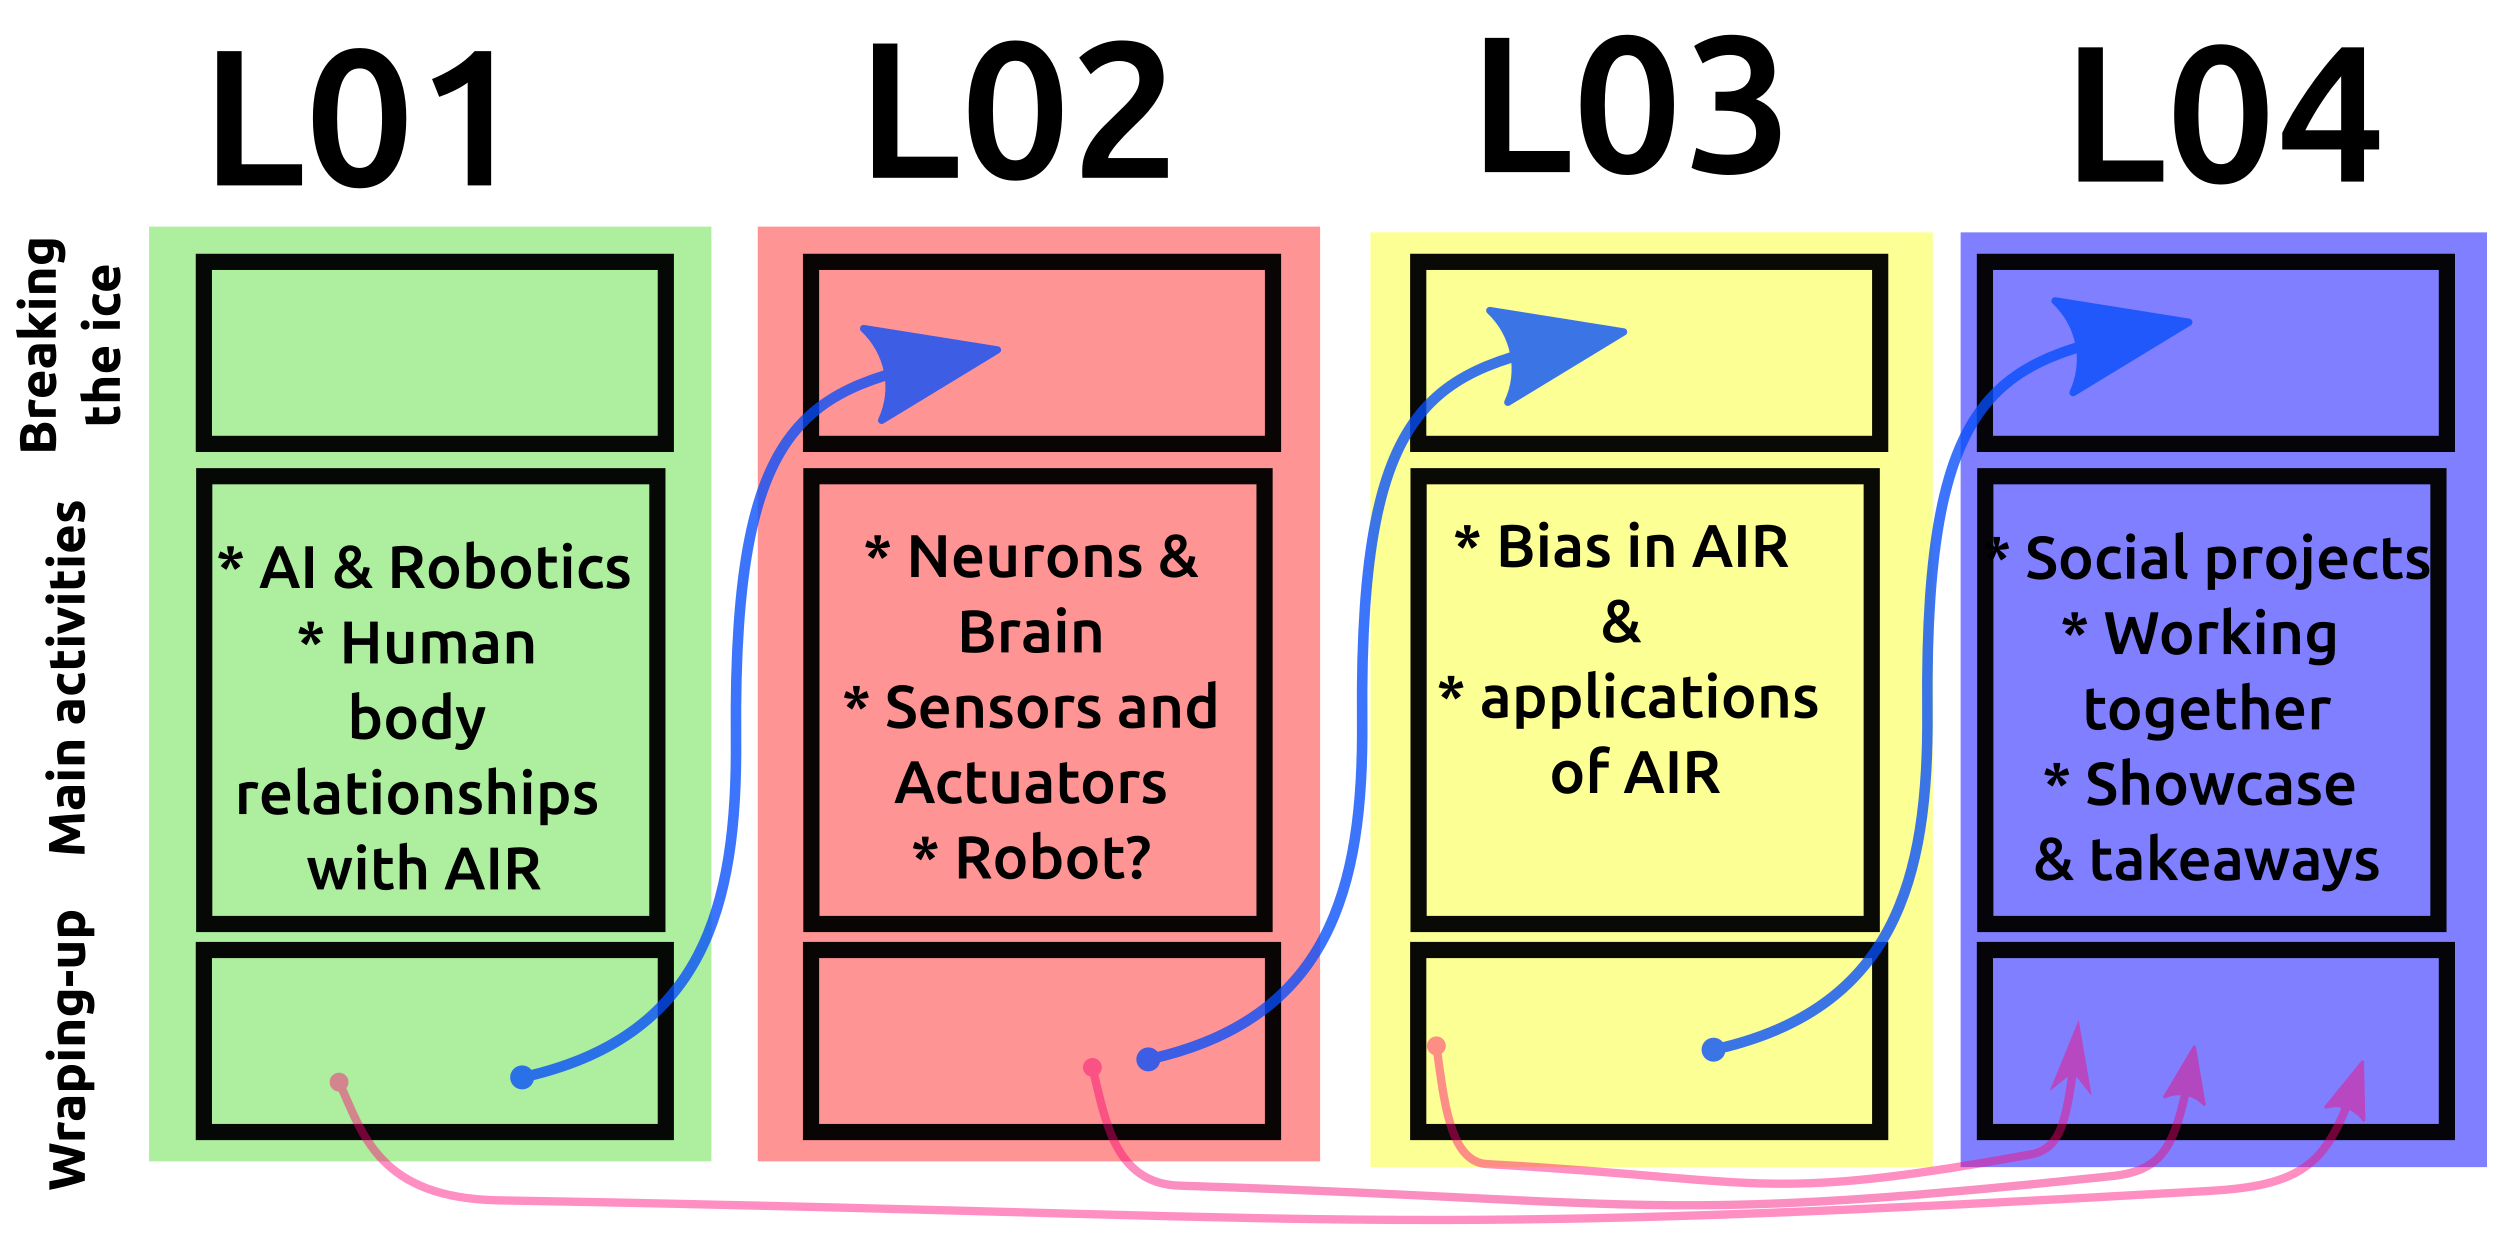
\includegraphics[width=1.0\textwidth]{curriculum/outputs/drawing-v00.png}
        %\caption{}
      \end{figure}
\end{frame}
}


%%%%%%%%%%%%%%%%%%%%%%%%%%%%%%%%%%%%%%%%%%%%%
\subsection{Piloting curriculum}



%%%%%%%%%%%%%%%%%%%%%%%%%%%%%%%%%%%%%%%%%%%%%%%%%%%%%%%%
{
\paper{Badillo-Perez A, Badillo-Perez D, Barco A, Montenegro R, \textbf{Xochicale M. 2023}, Teaching AI and Robotics to Children in a Mexican town, DEI-HRI2023, \url{https://arxiv.org/abs/2303.03956}}

\begin{frame}{Participants}

\begin{itemize}
\item 14 participants of which 10 were able to attend, 6 male and 4 female of (age in years: mean=8 and std=$\pm$1.61)     
\item Four instructors of different teaching experience levels to young audiences.
\end{itemize}

\end{frame}
}




%%%%%%%%%%%%%%%%%%%%%%%%%%%%%%%%%%%%%%%%%%%%%%%%%%%%%%%%
{
\paper{
      Badillo-Perez A, Badillo-Perez D, Barco A, Montenegro R, \textbf{Xochicale M. 2023}, Teaching AI and Robotics to Children in a Mexican town, DEI-HRI2023, \url{https://arxiv.org/abs/2303.03956}
      }

\begin{frame}{Piloting workshop: Coding and bingo activities}
      \begin{figure}
        \centering
        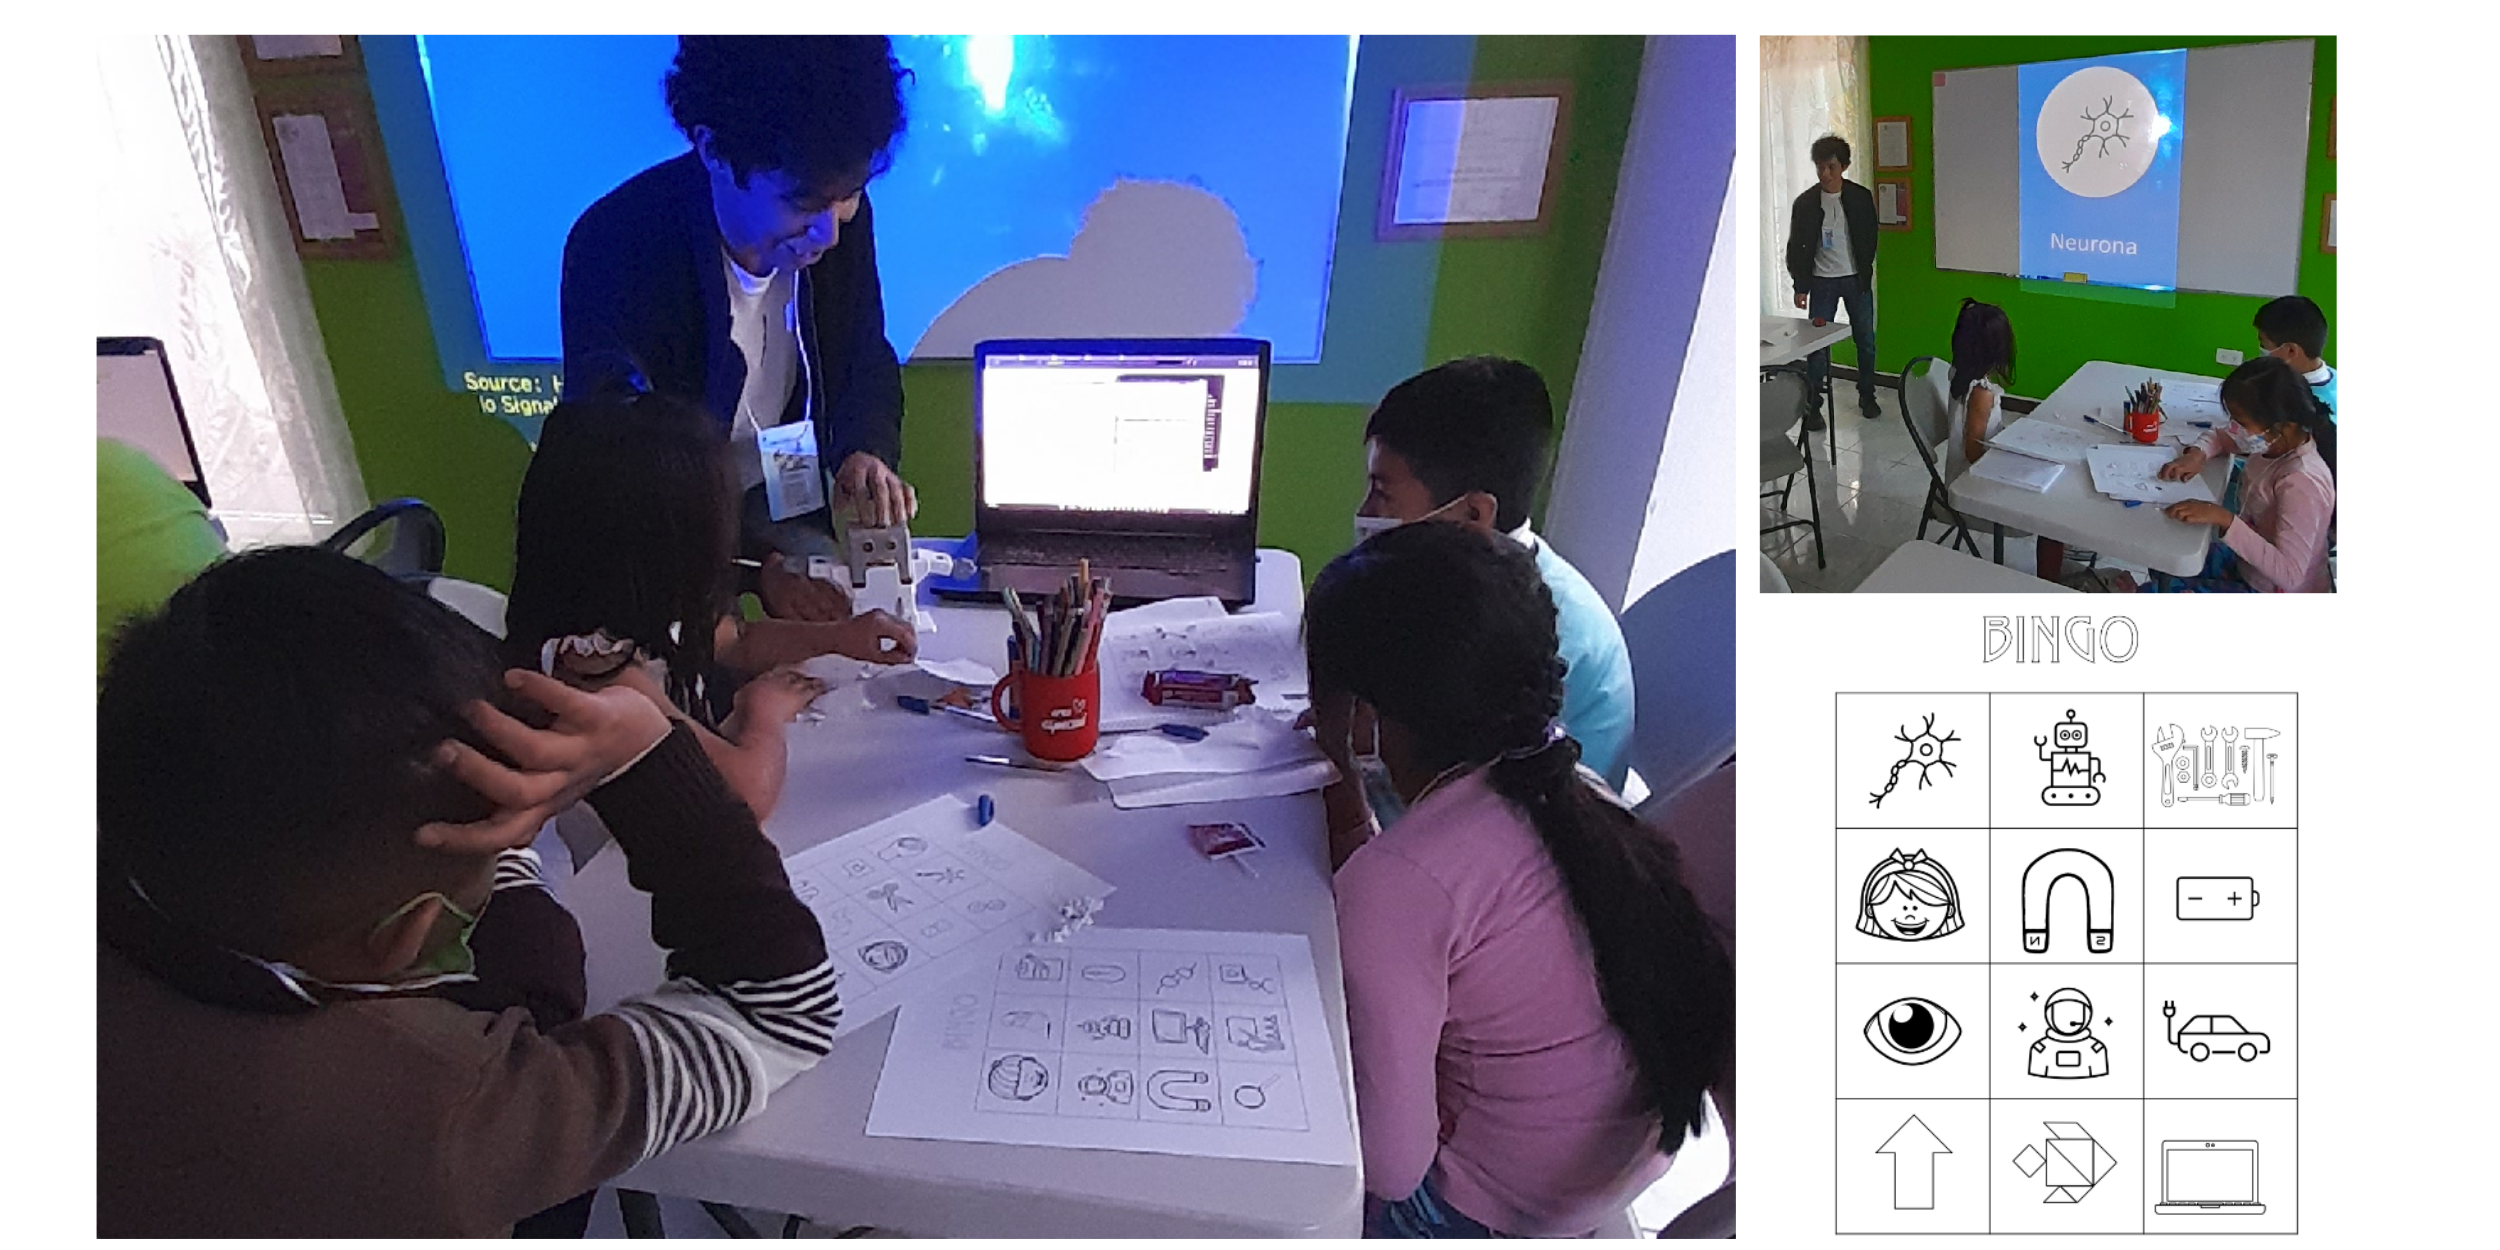
\includegraphics[width=1.0\textwidth]{pilot-workshop-a/outputs/drawing-v00.png}
        %\caption{}
      \end{figure}
\end{frame}
}



%%%%%%%%%%%%%%%%%%%%%%%%%%%%%%%%%%%%%%%%%%%%%%%%%%%%%%%%
{

\paper{Badillo-Perez A, Badillo-Perez D, Barco A, Montenegro R, \textbf{Xochicale M. 2023}, Teaching AI and Robotics to Children in a Mexican town, DEI-HRI2023, \url{https://arxiv.org/abs/2303.03956}}

\begin{frame}{Piloting workshop: Teaching activities}
      \begin{figure}
        \centering
        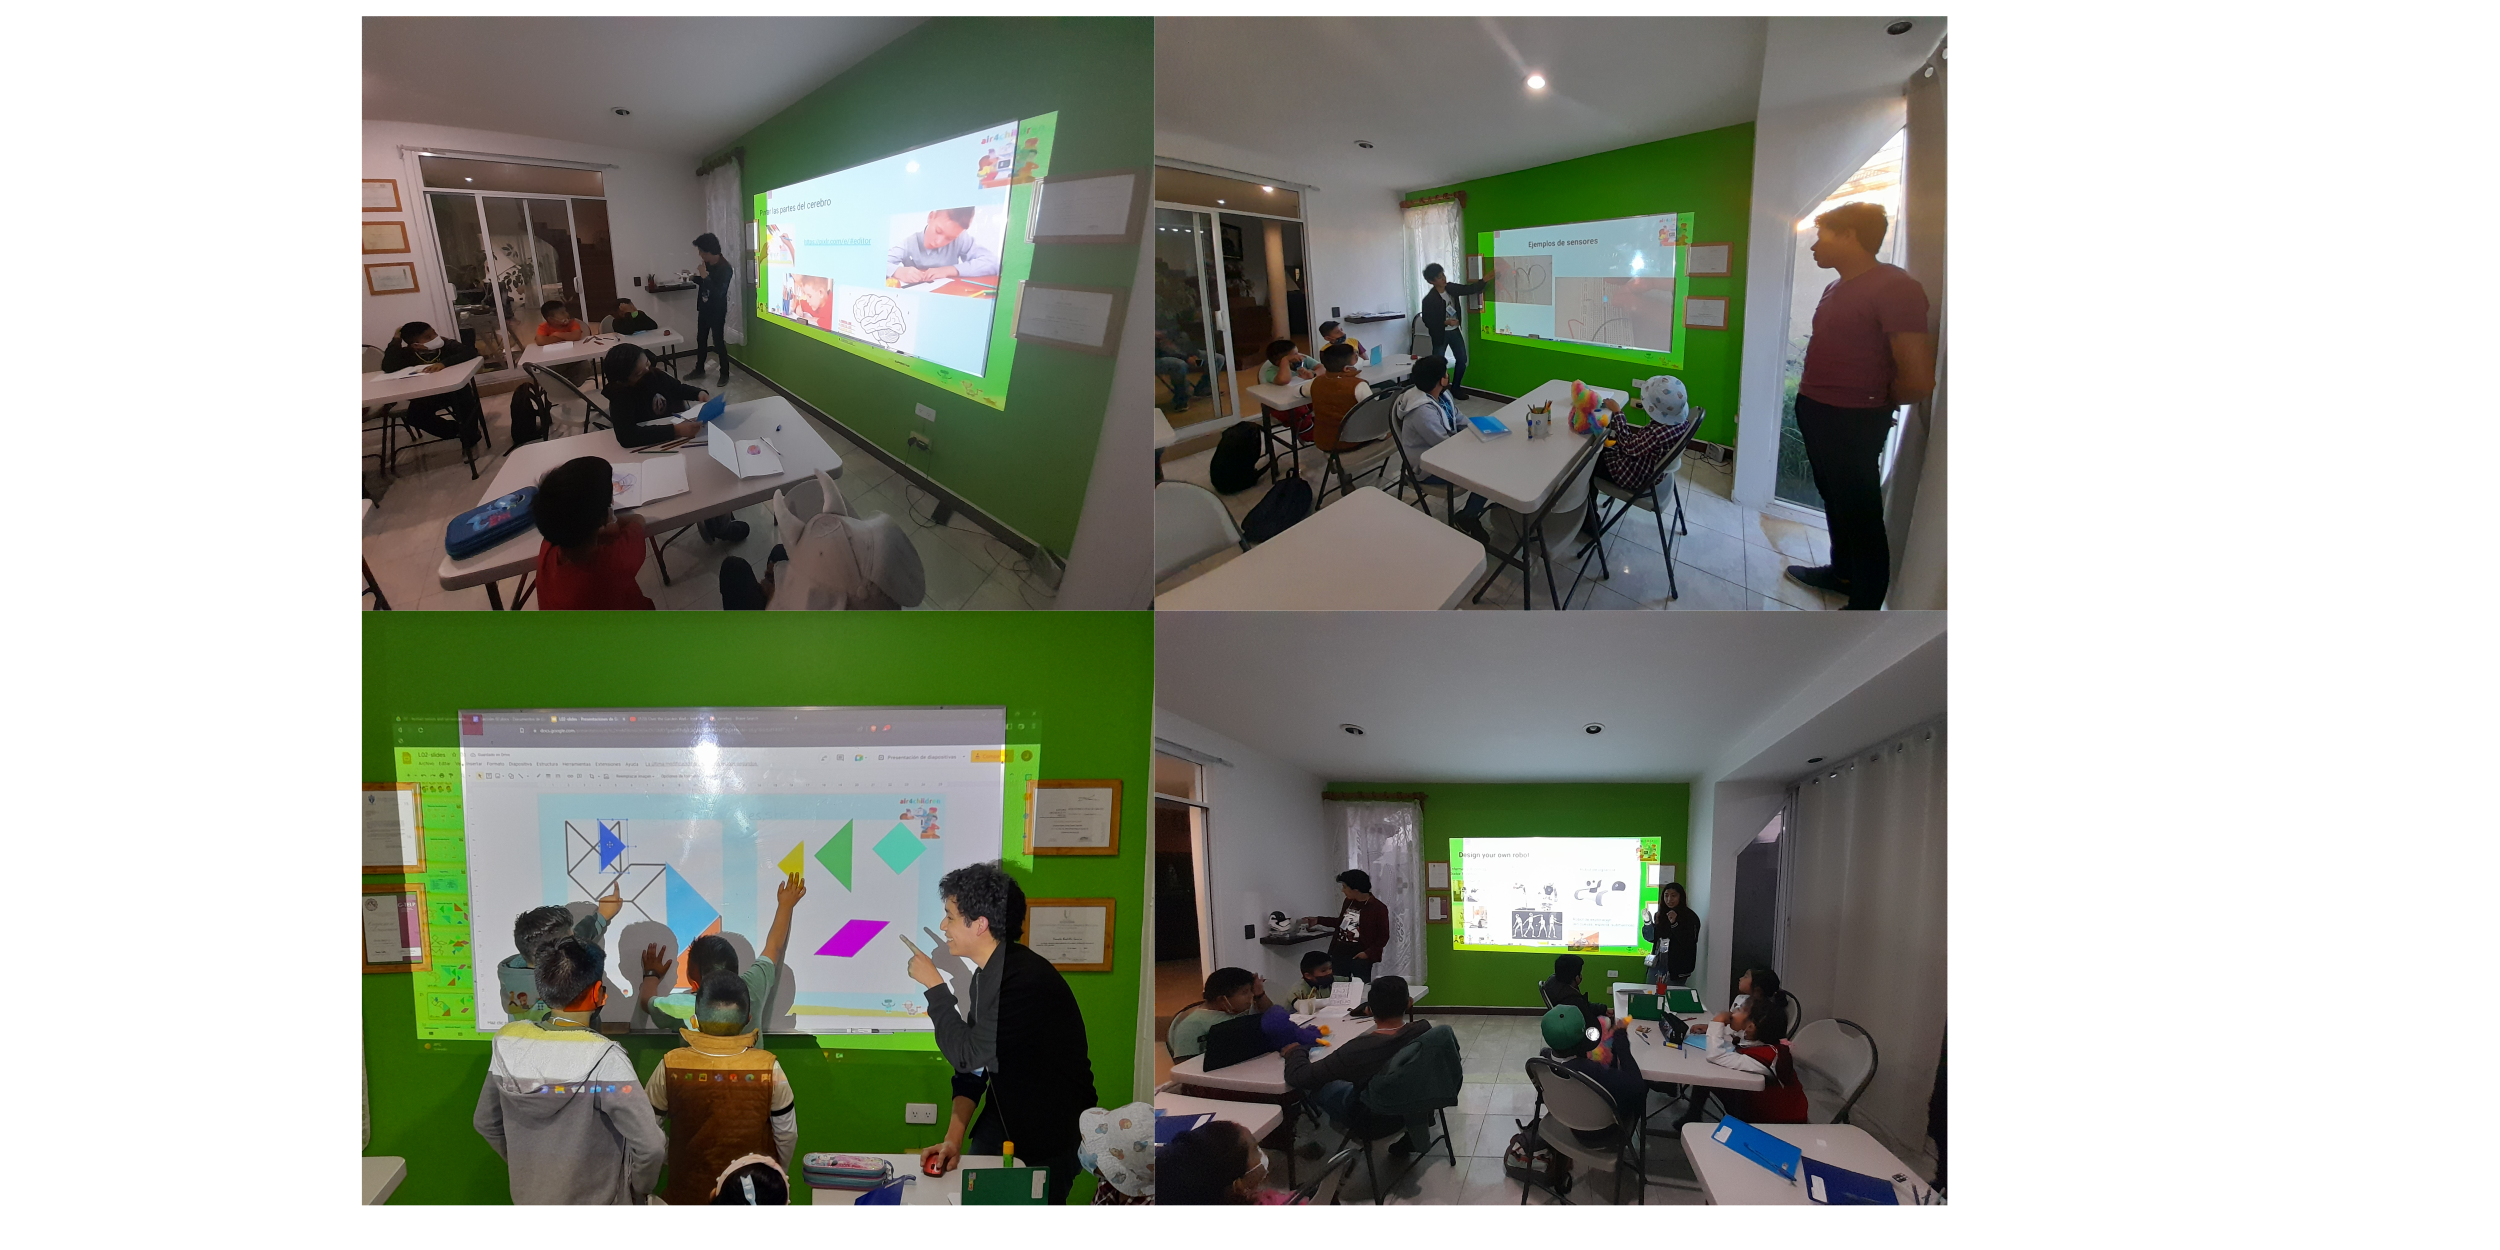
\includegraphics[width=1.0\textwidth]{pilot-workshop-b/outputs/drawing-v00.png}
        %\caption{}
      \end{figure}
\end{frame}
}

%%%%%%%%%%%%%%%%%%%%%%%%%%%%%%%%%%%%%%%%%%%%%%%%%%%%%%%%
{

\paper{Badillo-Perez A, Badillo-Perez D, Barco A, Montenegro R, \textbf{Xochicale M. 2023}, Teaching AI and Robotics to Children in a Mexican town, DEI-HRI2023, \url{https://arxiv.org/abs/2303.03956}}

\begin{frame}{Piloting workshop: Group activities}
      \begin{figure}
        \centering
        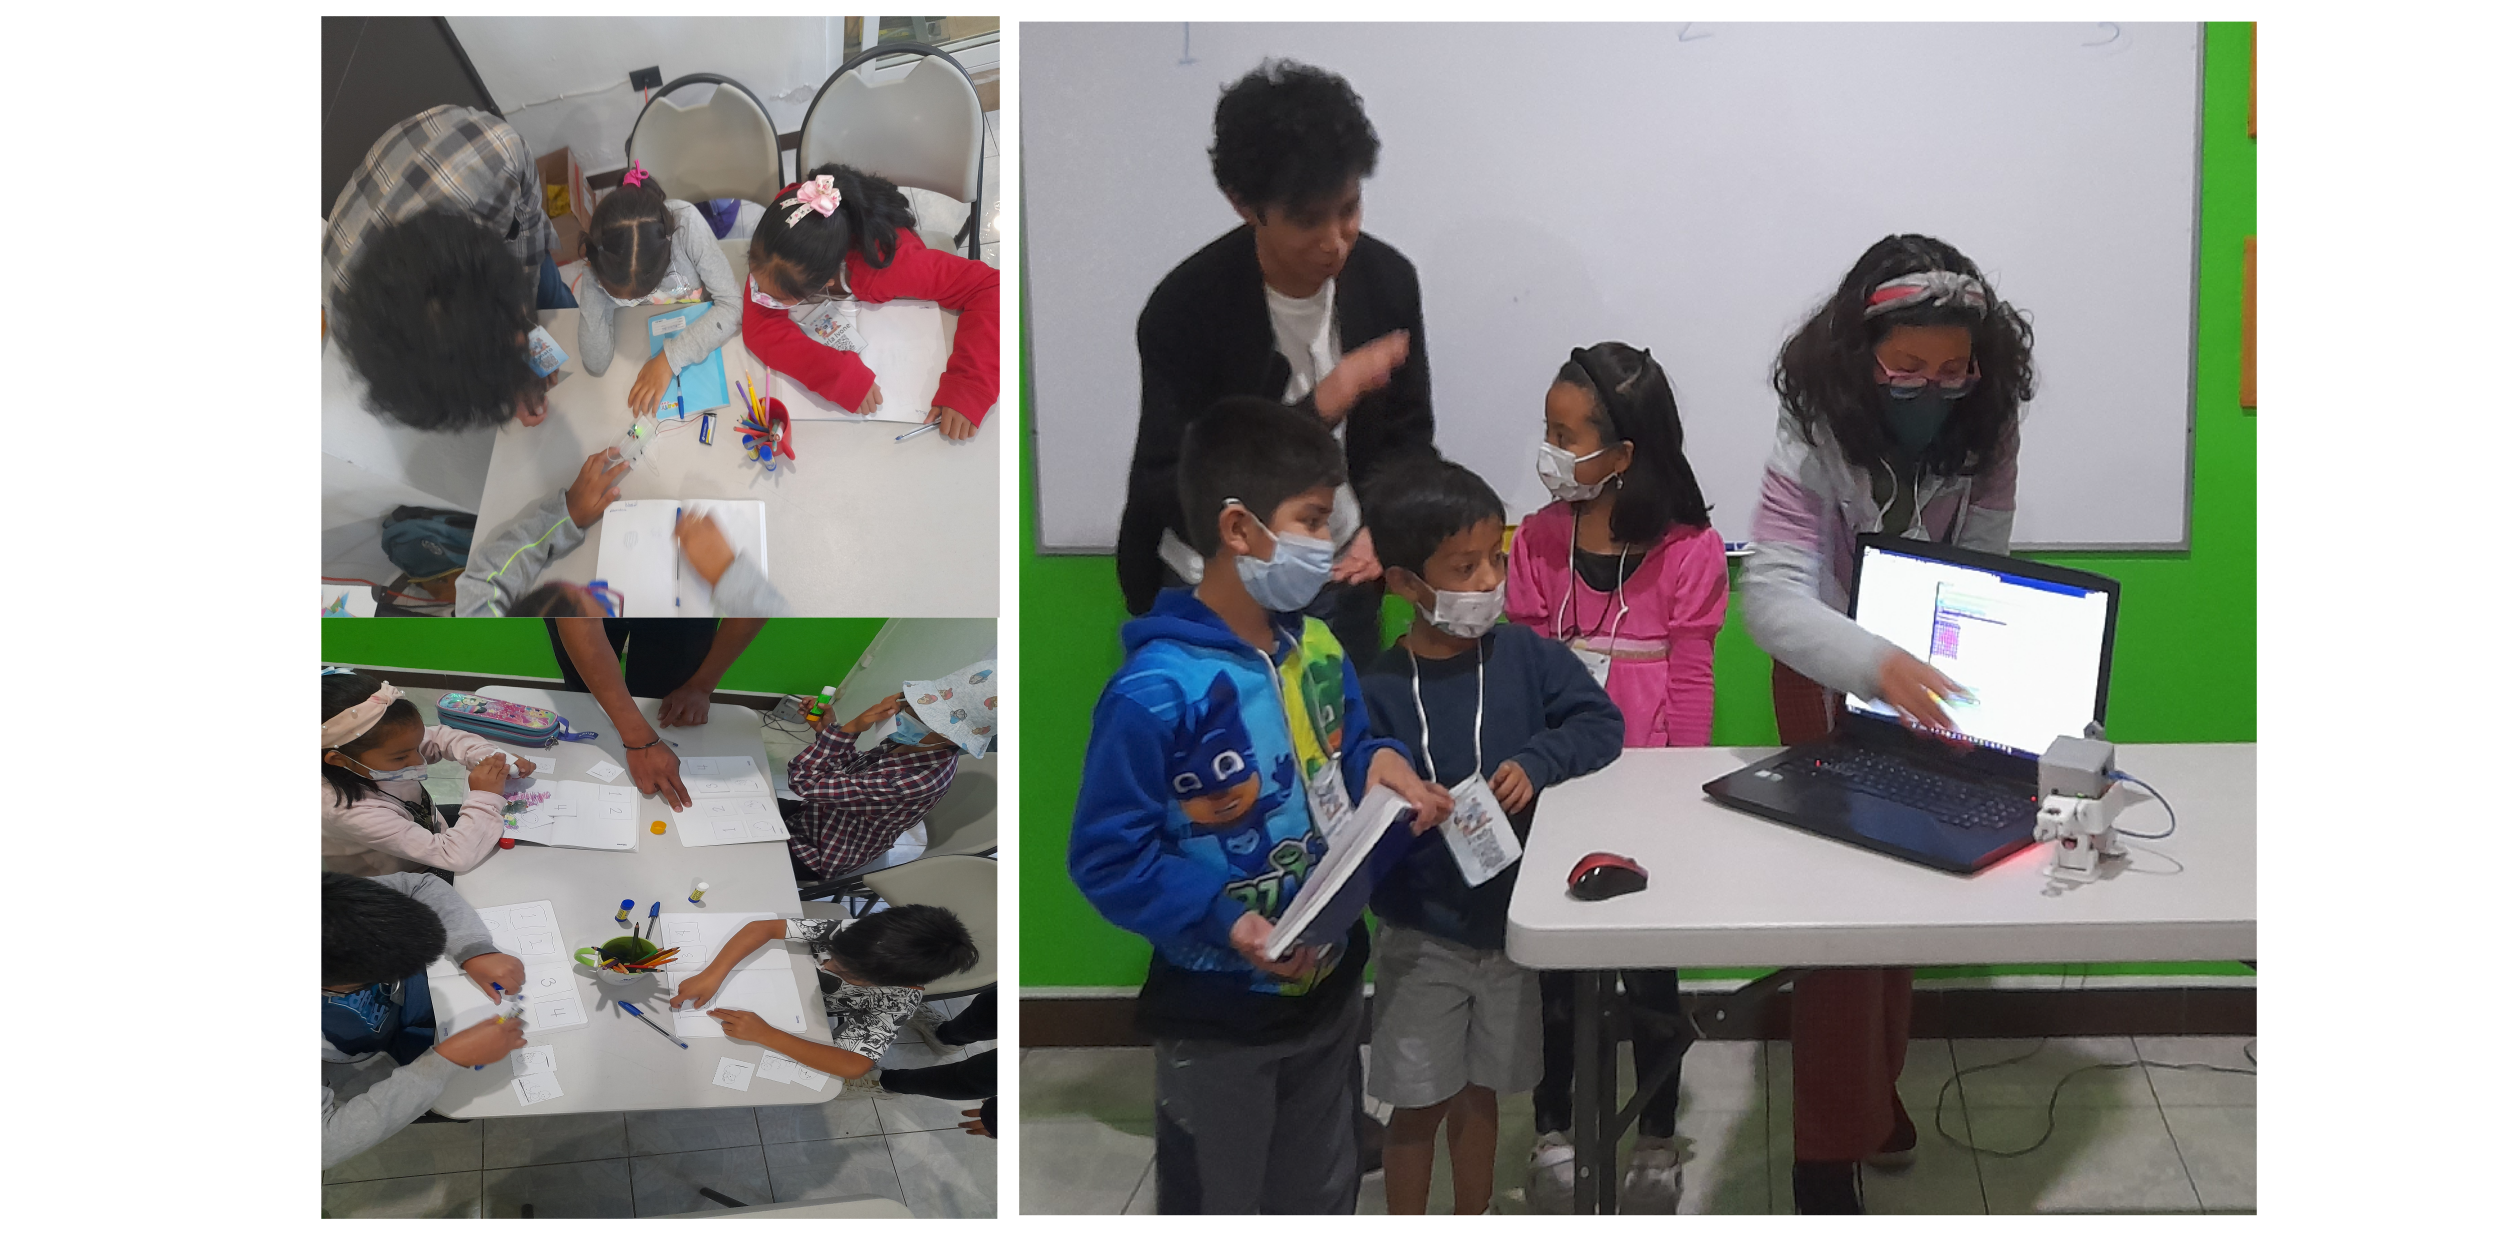
\includegraphics[width=1.0\textwidth]{pilot-workshop-c/outputs/drawing-v00.png}
        %\caption{}
      \end{figure}
\end{frame}
}

%%%%%%%%%%%%%%%%%%%%%%%%%%%%%%%%%%%%%%%%%%%%%
\subsection{Results of the survey}

%%%%%%%%%%%%%%%%%%%%%%%%%%%%%%%%%%%%%%%%%%%%%%%%%%%%%%%%
{

\paper{Badillo-Perez A, Badillo-Perez D, Barco A, Montenegro R, \textbf{Xochicale M. 2023}, Teaching AI and Robotics to Children in a Mexican town, DEI-HRI2023, \url{https://arxiv.org/abs/2303.03956}}

\begin{frame}{Survey results}
      \begin{figure}
        \centering
        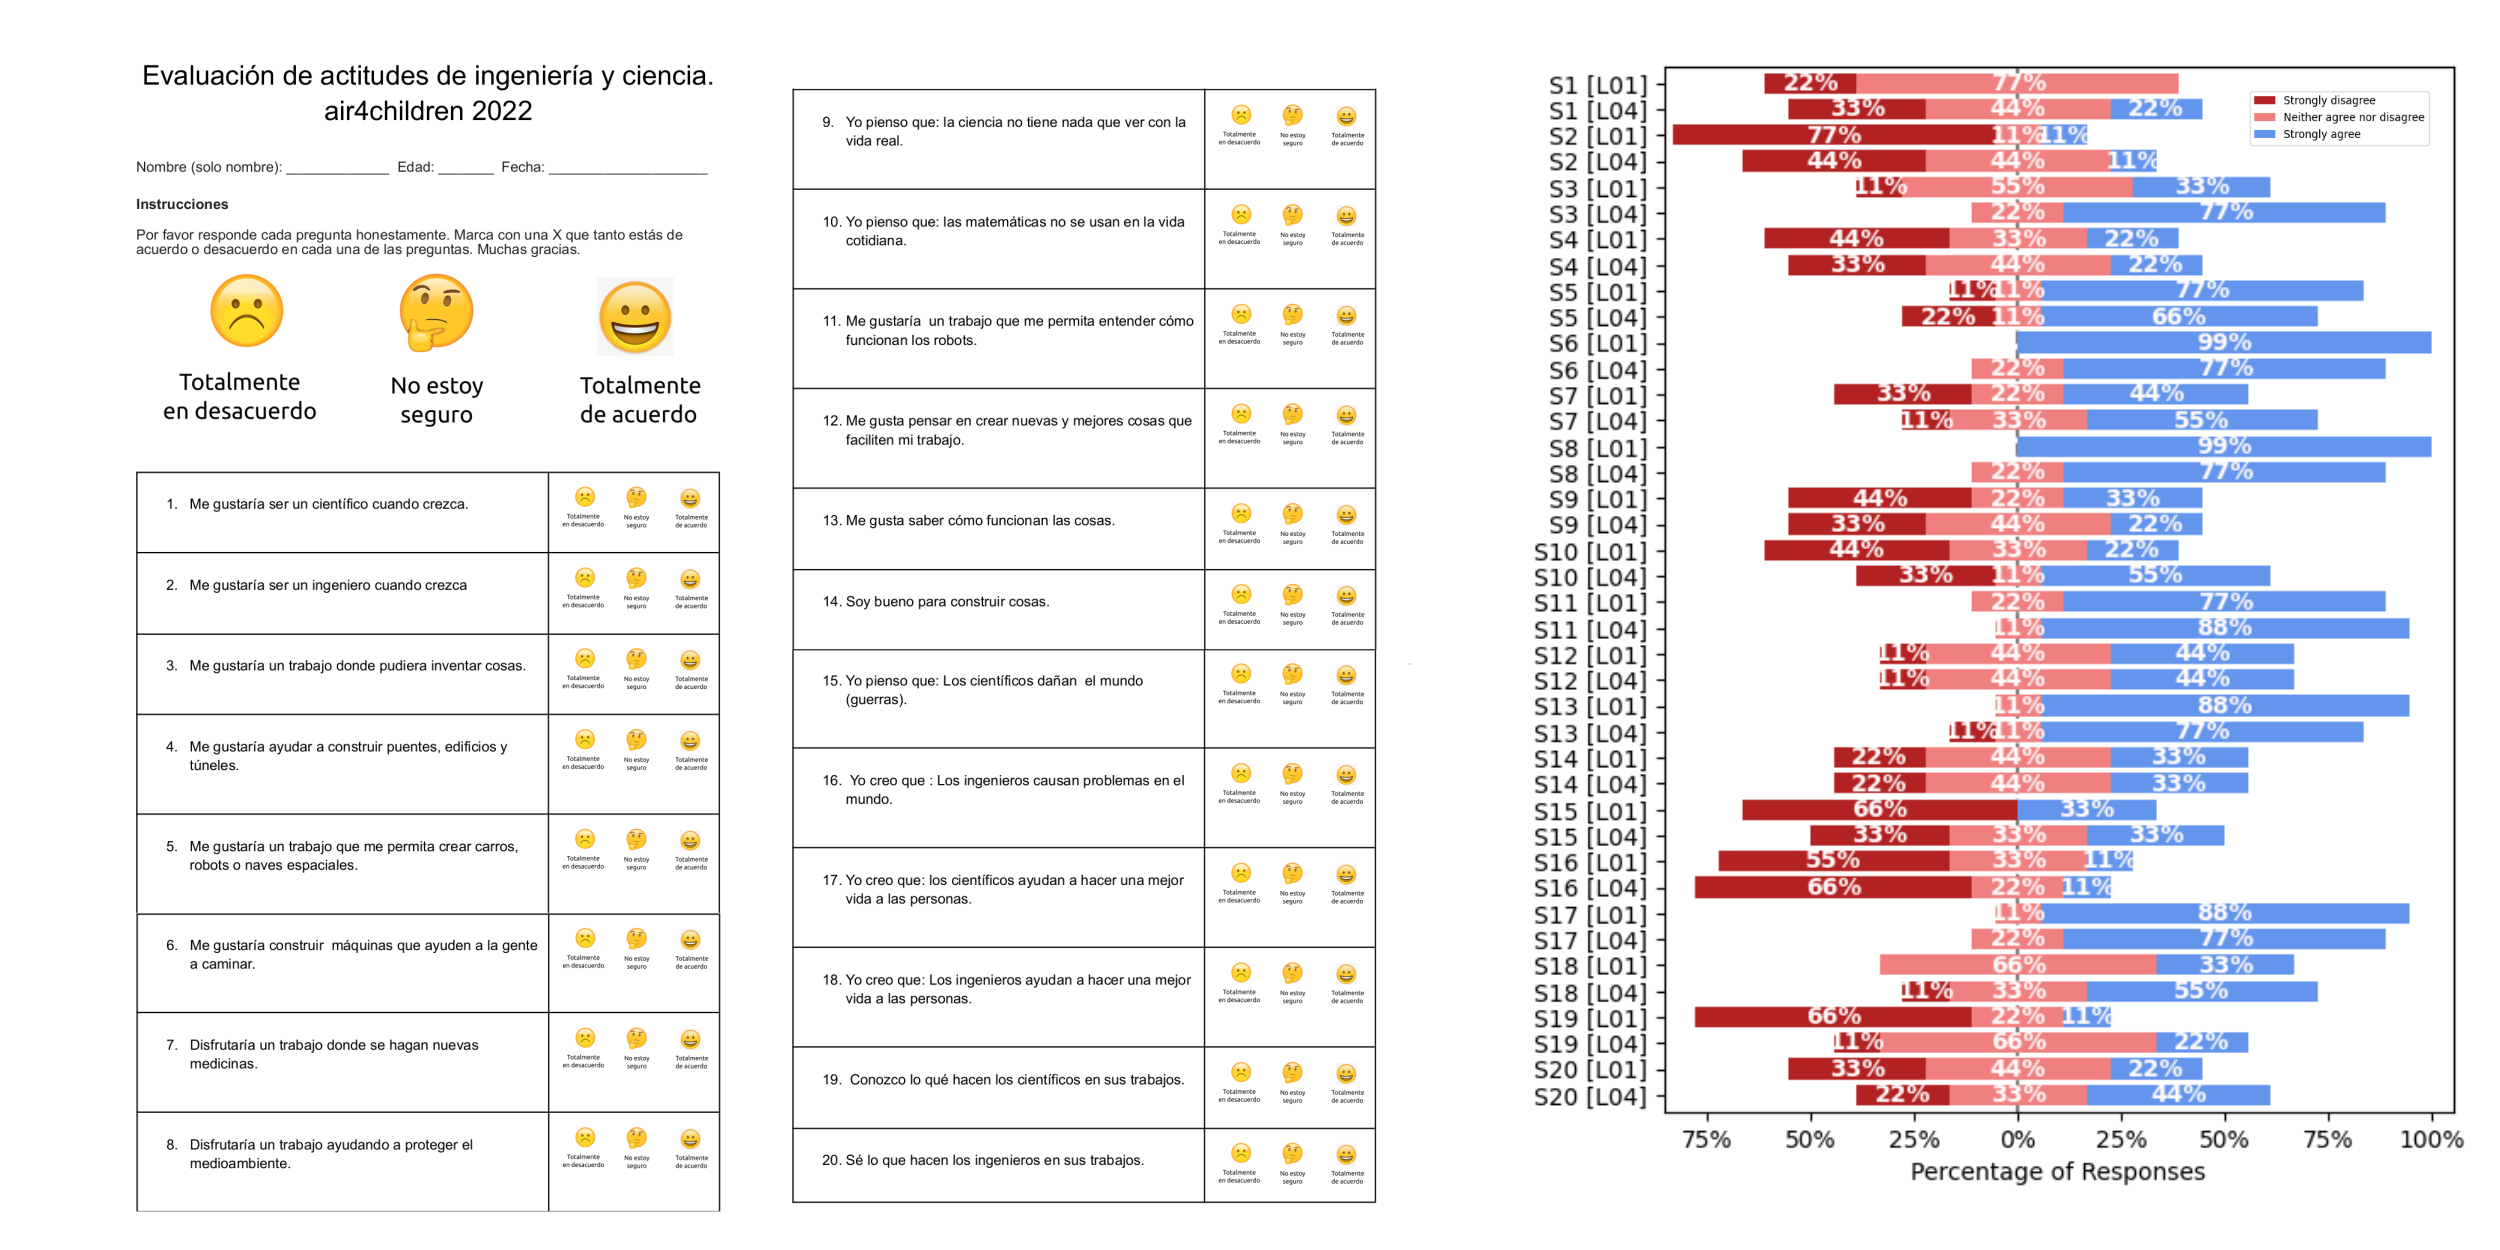
\includegraphics[width=1.0\textwidth]{survey-results/outputs/drawing-v00.png}
        %\caption{}
      \end{figure}
\end{frame}
}



%%%%%%%%%%%%%%%%%%%%%%%%%%%%%%%%%%%%%%%%%%%%%%%%%%%%%%%%
{
\paper{Badillo-Perez A, Badillo-Perez D, Barco A, Montenegro R, \textbf{Xochicale M. 2023}, Teaching AI and Robotics to Children in a Mexican town, DEI-HRI2023, \url{https://arxiv.org/abs/2303.03956}}

\begin{frame}{Statistical analysis}

\begin{itemize}
\item A Wilcoxon T test was used to analyze the results of the survey before and after the survey to see if the engineering attitudes had a significant effect on pre and post survey of the workshop.
\item The average survey before the test was lower ($\mu$ = 2.194500 $\pm \sigma$ 0.558367 ) compared to the posttest results ($\mu$ = 2.239500 $\pm \sigma$= 0.396796).
\item There was no statistically significant in the increase of attitudes towards engineering (t=53.5, p= 0.45).
\end{itemize}

See Appendix section for reproducible Jupyter notebooks of statistical analysis and plots.

\end{frame}
}





%%%%%%%%%%%%%%%%%%%%%%%%%%%%%%%%%%%%%%%%%%%%
\section{Conclusions and Future work}


\begin{frame}
      \frametitle{Table of Contents}
      \tableofcontents[currentsection]
\end{frame}



%%%%%%%%%%%%%%%%%%%%%%%%%%%%%%%%%%%%%%%%%%%%%%%%%%%%%%%%
{
%\paper{Lastname N. YEAR in journal of...}
\begin{frame}{Conclusions and future work}

  \begin{columns}
  \begin{column}{.75\linewidth}

  \textbf{Conclusions}   

  \begin{itemize}
    \item Applied Montessory Education and spiral education to design child-based curriculumns in AI and Robotics
    \item Piloted a workshop with 14 participants of 4 lessons surveying attitudes with liker chart
  \end{itemize}

  \textbf{Future work}
  \begin{itemize}
    \item Improve surveys and statistical analysis
    \item Piloting AIR4Children with a major number of participants 
    \item Applying for funding 
    \item Engage with policy makers to increase the impact of air4children
\end{itemize}

    \end{column}


  \begin{column}{.3\linewidth}

      \begin{figure}
        \centering
        
\includegraphics[width=0.9\textwidth]{logo/outputs/drawing-v00.png}
      \end{figure}

    \end{column}
  \end{columns}

\end{frame}
}


%%%%%%%%%%%%%%%%%%%%%%%%%%%%%%%%%%%%%%%%%%%%%%%%%%%%%%%%%
%{
%%\paper{Lastname N. YEAR in journal of...}
%\begin{frame}{Acknowledgements}
%
%  \begin{figure}
%  \centering
%  
\includegraphics[width=1.0\textwidth]{./figures/team/outputs/drawing-v00.png}
%  \end{figure}
%
%\end{frame}
%}
%



%\begin{frame}
%  Thanks \\
%  Questions?
%\end{frame}

\maketitle

\end{document}
